%%____________________________________________________________________________||
\section{Interpretation in Simplified SUSY models}
\label{sec:susy}
To interpret the results of this search, simplified
models~\cite{Alwall:2008ag,Alwall:2008va,sms} for the production of supersymmetric particles are considered. 
They use only a limited set of sparticles in the production and
decay and enable comprehensive studies of individual SUSY event
topologies. These studies can be performed in terms of
fundamental properties such as decay modes, production cross sections and sparticle masses. 
In order to gauge the early discovery potential, simplified models corresponding to both gluino and squark pair production 
are considered in this exercise, corresponding to different scenarios for the mass-splitting between the sparticle and the LSP. 

\subsection{Signal models and efficiencies}
\label{subsec:susy_models}

The full list of models considered is in table \ref{tab:simplified-models}. 
The signal efficiency times acceptance is determined per model per event
category (\njet,\nb) per \HT bin. 
Systematic uncertainties on the signal efficiencies are determined 
following the 2012 analysis (see Section~\ref{sec:sig-syst}). Due to CPU
limitations, only a subset of event categories (but all \scalht bins
within a category) are considered to extract the final result. 
The categories included in the fit are the ten most sensitive 
for each model and are listed in table \ref{tab:simplified-models}. 

\begin{landscape}

\begin{table}[h!]
  \caption{A summary of the simplified benchmark models considered in 
    this exercise. The models labelled as ``T1'' correspond to the pair production of gluinos, while 
    those labelled as ``T2'' correspond to the pair production of squarks (stop, sbottom or degenerate light flavour). 
    The event categories considered for each model are listed. 
    For the jet multiplicity categorisation, the ``$j$'' refers to the ``symmetric'' selection, while ``$a$'' refers to the ``asymmetric'' one.}  
  \label{tab:simplified-models}
  %% \setlength{\extrarowheight}{2.5pt}
  \centering
  %% \begin{tabular*}{\textwidth}{ llcc }
  \begin{tabular*}{1.4\textwidth}{ llcl }
    \hline
    \hline
    %% Model & Production/decay mode & ($m_{\rm SUSY},m_{\rm LSP}$) [GeV] & (\njet,\nb) event categories \\ 
    Model & Production/decay mode & ($m_{\rm SUSY},m_{\rm LSP}$) [GeV] & (\nb,\njet) event categories \\ 
    \hline    
    \multirow{2}{*}{T1bbbb 1500,100} & \multirow{2}{*}{\Tonebbbb} & \multirow{2}{*}{(1500,100)} & {\small $ (2b,\geq5j), (\geq3b,\geq5j), (1b,\geq5j), (2b,\geq5a)$} \\
    & & & {\small $ (2b,4j), (1b,4j), (\geq3b,\geq5a), (2b,4a), (1b,3a), (2b,3j)$} \\ \hline
    \multirow{2}{*}{T1bbbb 1000,900} & \multirow{2}{*}{\Tonebbbb} & \multirow{2}{*}{(1000,900)} & {\small $ (2b,\geq5j), (\geq3b,\geq5j), (1b,\geq5j), (2b,\geq5a)$} \\
    & & & {\small $ (2b,4j), (1b,4j), (\geq3b,\geq5a), (2b,4a), (1b,3a), (2b,3j)$} \\ \hline
    \multirow{2}{*}{T1qqqq 1400,100} & \multirow{2}{*}{\Toneqqqq} & \multirow{2}{*}{(1400,100)} & {\small $ (0b,\geq5j), (1b,\geq5j), (0b,4j), (2b,\geq5j)$} \\
    & & & {\small $ (1b,4j), (0b,3j), (2b,4j), (\geq3b,\geq5j), (1b,3j), (2b,3j)$} \\ \hline
    \multirow{2}{*}{T1qqqq 1000,800} & \multirow{2}{*}{\Toneqqqq} & \multirow{2}{*}{(1000,800)} & {\small $ (0b,\geq5j), (1b,\geq5j), (0b,4j), (0b,\geq5a)$} \\
    & & & {\small $ (2b,\geq5j), (1b,4j), (0b,4a), (0b,3j), (0b,3a), (\geq3b,\geq5j)$} \\ \hline
    \multirow{2}{*}{T1tttt 1500,100} & \multirow{2}{*}{\Tonetttt} & \multirow{2}{*}{(1500,100)} & {\small $ (\geq3b,\geq5j), (2b,\geq5j), (1b,\geq5j), (0b,\geq5j)$} \\
    & & & {\small $ (2b,4j), (1b,4j), (\geq3b,4j), (2b,3j), (1b,\geq5a), (0b,4j)$} \\ \hline
    \multirow{2}{*}{T1tttt 1200,800} & \multirow{2}{*}{\Tonetttt} & \multirow{2}{*}{(1200,800)} & {\small $ (\geq3b,\geq5j), (2b,\geq5j), (\geq3b,\geq5a), (1b,\geq5j)$} \\
    & & & {\small $ (2b,\geq5a), (1b,\geq5a), (0b,\geq5j), (0b,\geq5a), (2b,4j), (\geq3b,4j)$} \\ \hline
    \hline
    \multirow{2}{*}{T2tt 650,325}    & \multirow{2}{*}{\Ttwott}   & \multirow{2}{*}{(650,550)} & {\small $ (1b,\geq5j), (\geq3b,\geq5j), (2b,4j), (2b,\geq5a)$} \\
    & & & {\small $ (1b,4j), (0b,\geq5j), (2b,4a), (\geq3b,\geq5a), (1b,4a), (1b,3j)$} \\ \hline
    \multirow{2}{*}{T2tt 500,325}    & \multirow{2}{*}{\Ttwott}   & \multirow{2}{*}{(500,325)} & {\small $ (1b,\geq5j), (2b,\geq5j), (\geq3b,\geq5j), (2b,\geq5a)$} \\
    & & & {\small $ (0b,\geq5j), (1b,4j), (\geq3b,\geq5a), (2b,4j), (0b,\geq5a), (1b,4a)$} \\ \hline
    \multirow{2}{*}{T2tt 425,325}    & \multirow{2}{*}{\Ttwott}   & \multirow{2}{*}{(425,325)} & {\small $ (0b,\geq5j), (1b,\geq5j), (0b,\geq5a), (0b,4j)$} \\
    & & & {\small $ (2b,\geq5j), (1b,4j), (0b,4a), (0b,3j), (1b,4a), (0b,3a)$} \\ \hline
    \multirow{2}{*}{T2qq 600,550}    & \multirow{2}{*}{\Ttwoqq}   & \multirow{2}{*}{(600,550)} & {\small $ (0b,\geq5j), (1b,\geq5j), (0b,4j), (0b,\geq5a)$} \\
    & & & {\small $ (0b,4a), (0b,3j), (0b,3a), (1b,4j), (2b,\geq5j), (1b,4a)$} \\ \hline
    \multirow{2}{*}{T2qq 1200,100}   & \multirow{2}{*}{\Ttwoqq}   & \multirow{2}{*}{(1200,100)} & {\small $ (0b,\geq5j), (0b,4j), (0b,3j), (0b,2j)$} \\
    & & & {\small $ (1b,\geq5j), (1b,4j), (1b,3j), (1b,2j), (2b,\geq5j), (2b,4j)$} \\ \hline
    \multirow{2}{*}{T2bb 900,100}    & \multirow{2}{*}{\Ttwobb}   & \multirow{2}{*}{(900,100)} & {\small $ (2b,3j), (2b,2j), (2b,\geq5j), (2b,4j)$} \\
    & & & {\small $ (1b,2j), (1b,\geq5j), (1b,3j), (1b,4j), (\geq3b,\geq5j), (0b,\geq5j)$} \\ \hline
    \multirow{2}{*}{T2bb 600,580}    & \multirow{2}{*}{\Ttwobb}   & \multirow{2}{*}{(600,580)} & {\small $ (1b,\geq5j), (0b,\geq5j), (0b,3j), (0b,4j)$} \\
    & & & {\small $ (1b,4j), (1b,3j), (0b,2j), (2b,\geq5j), (0b,3a), (0b,2a)$} \\ 
    \hline
    \hline
  \end{tabular*}
\end{table}

\end{landscape}

\subsection{Systematic uncertainties on signal efficiency times acceptance}
\label{sec:sig-syst}

For these results the same systematic uncertainty on the signal yield 
as in the previous Run 1 analysis is assumed \cite{CMS_AN_2013-366}. 
The following sources of uncertainty were considered: 
luminosity, parton distribution
functions, jet energy scale, initial state radiation, 
efficiencies of the \mht/\met filter and ``dead ECAL'' filter. 
Each contribution is considered to be independent and all contributions are
summed in quadrature. \\
A flat 15\% uncertainty is applied, fully correlated across all the bins (see Section \ref{sec:likelihood}). 
The uncorrelated approach has been checked to give very similar results. \\
No shape uncertainty for the signal is considered in these results, 
but dedicated studies will be carried on in the future about this.


\subsection{Expected exclusion limits and discovery significance}
\label{subsec:susy_results}

In order to extract the signal contribution in the fit, the distribution of events according to the \mht variable, 
encoded as template histograms, is used as described in Sections \ref{sec:had-shape} and \ref{sec:likelihood}. \\
The \mht templates histograms for the backgrounds together with some benchmark models are shown in Figures ~\ref{fig:mht_eq0b_eq4j},\ref{fig:mht_eq0b_ge5j},\ref{fig:mht_eq0b_ge5a},\ref{fig:mht_eq1b_ge5j},\ref{fig:mht_eq2b_ge5a},\ref{fig:mht_ge3b_ge5j} for the most relevant \HT bins. 

\begin{figure}
  \begin{center}
    \subfigure[$350 < \HT < 400  \gev$]{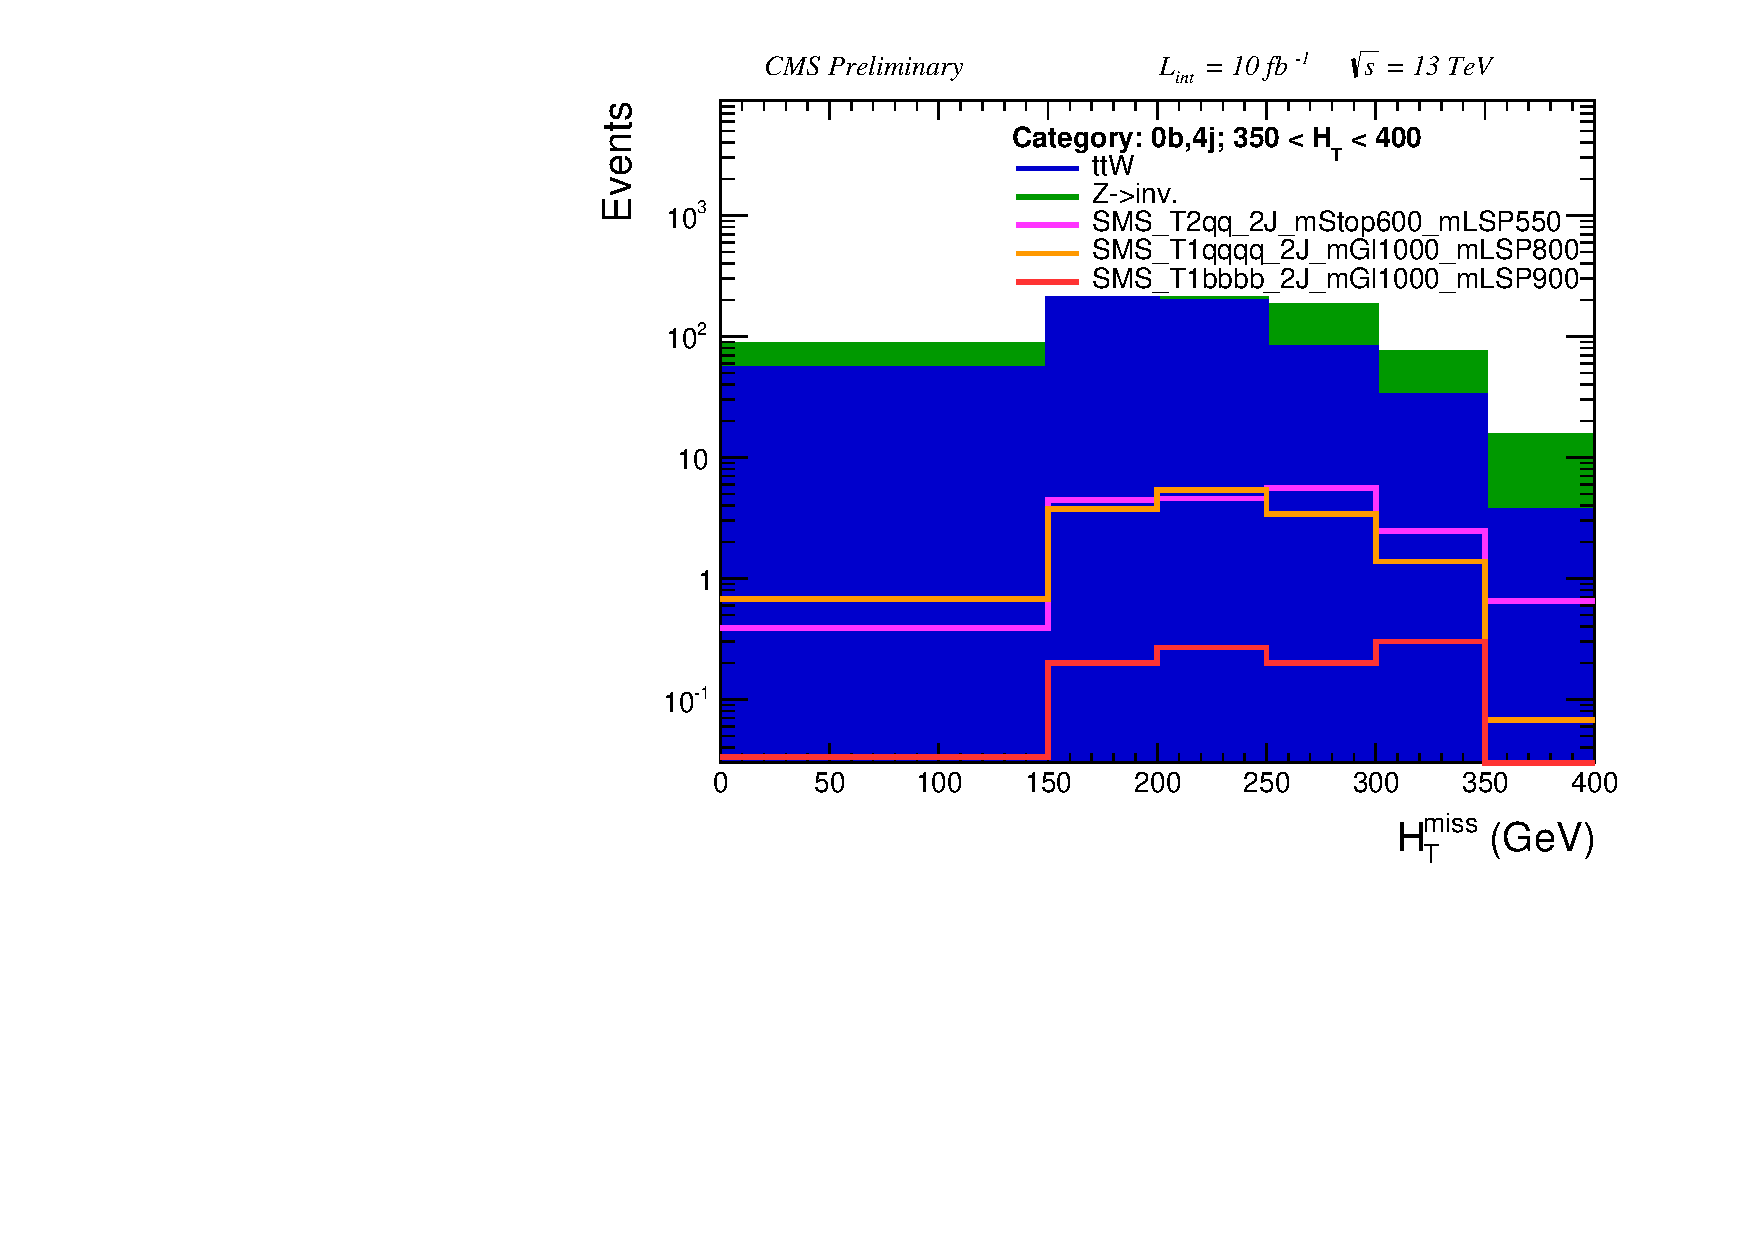
\includegraphics[width=0.5\textwidth]{figures/susyResults/MHT_eq0b_eq4j_350_400.pdf}} ~~
    \subfigure[$400 < \HT < 600  \gev$]{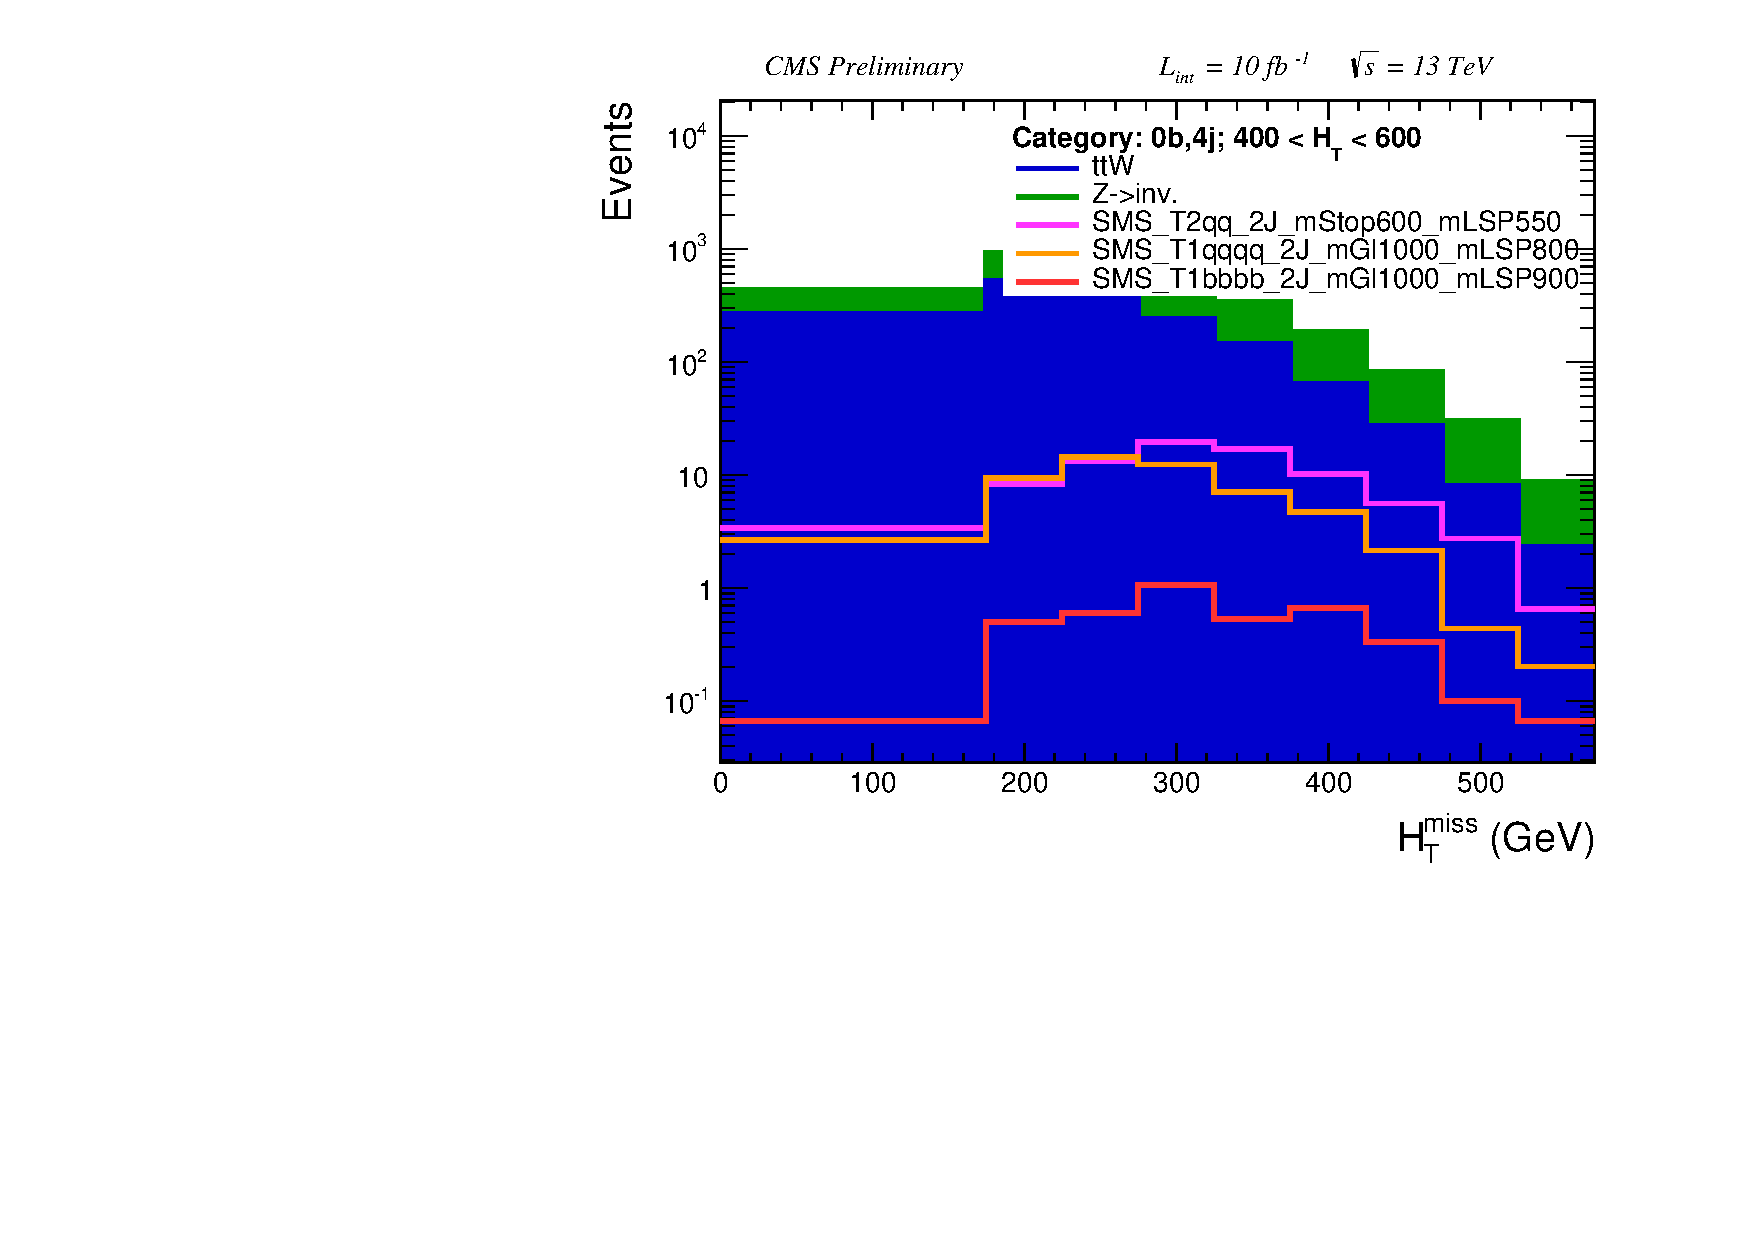
\includegraphics[width=0.5\textwidth]{figures/susyResults/MHT_eq0b_eq4j_400_600.pdf}} \\
    \subfigure[$600 < \HT < 800  \gev$]{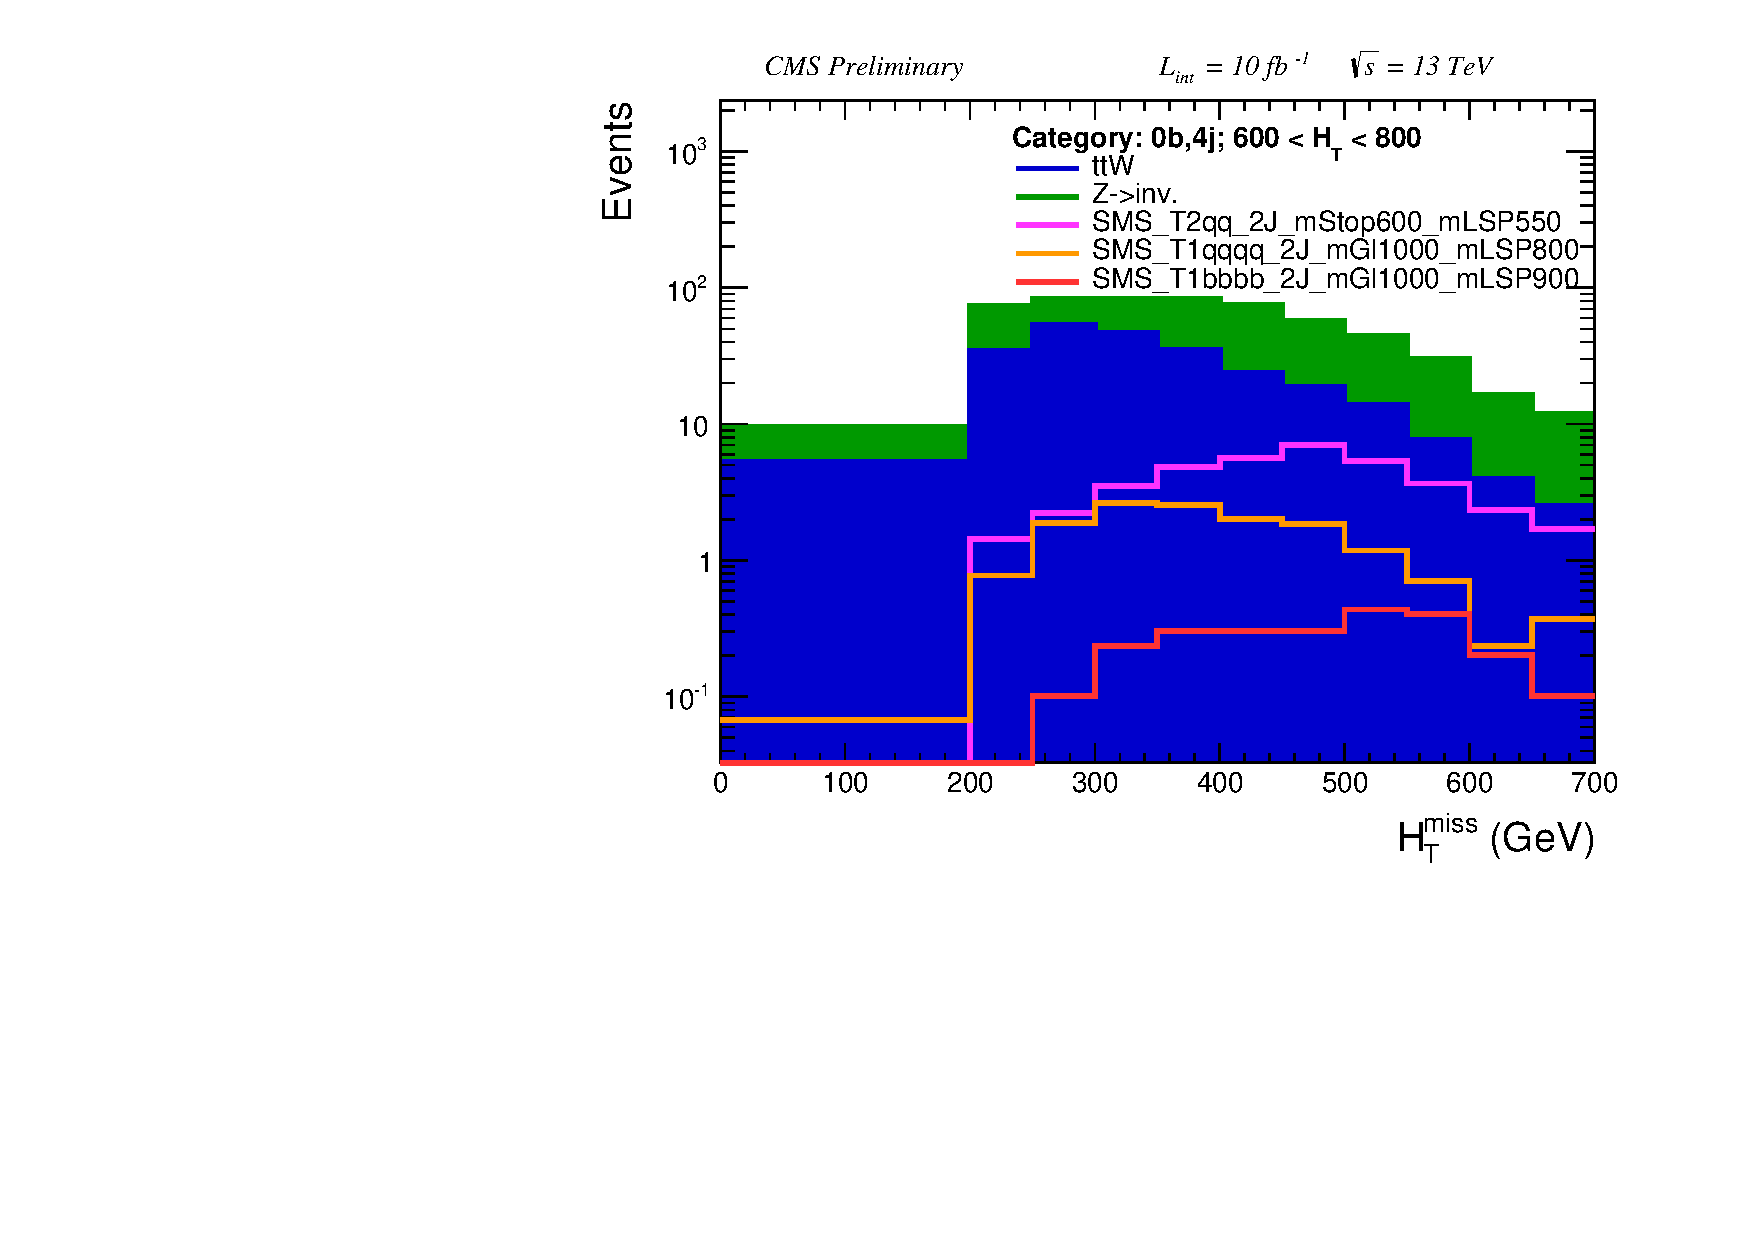
\includegraphics[width=0.5\textwidth]{figures/susyResults/MHT_eq0b_eq4j_600_800.pdf}} ~~
    \subfigure[$\HT > 800  \gev$]{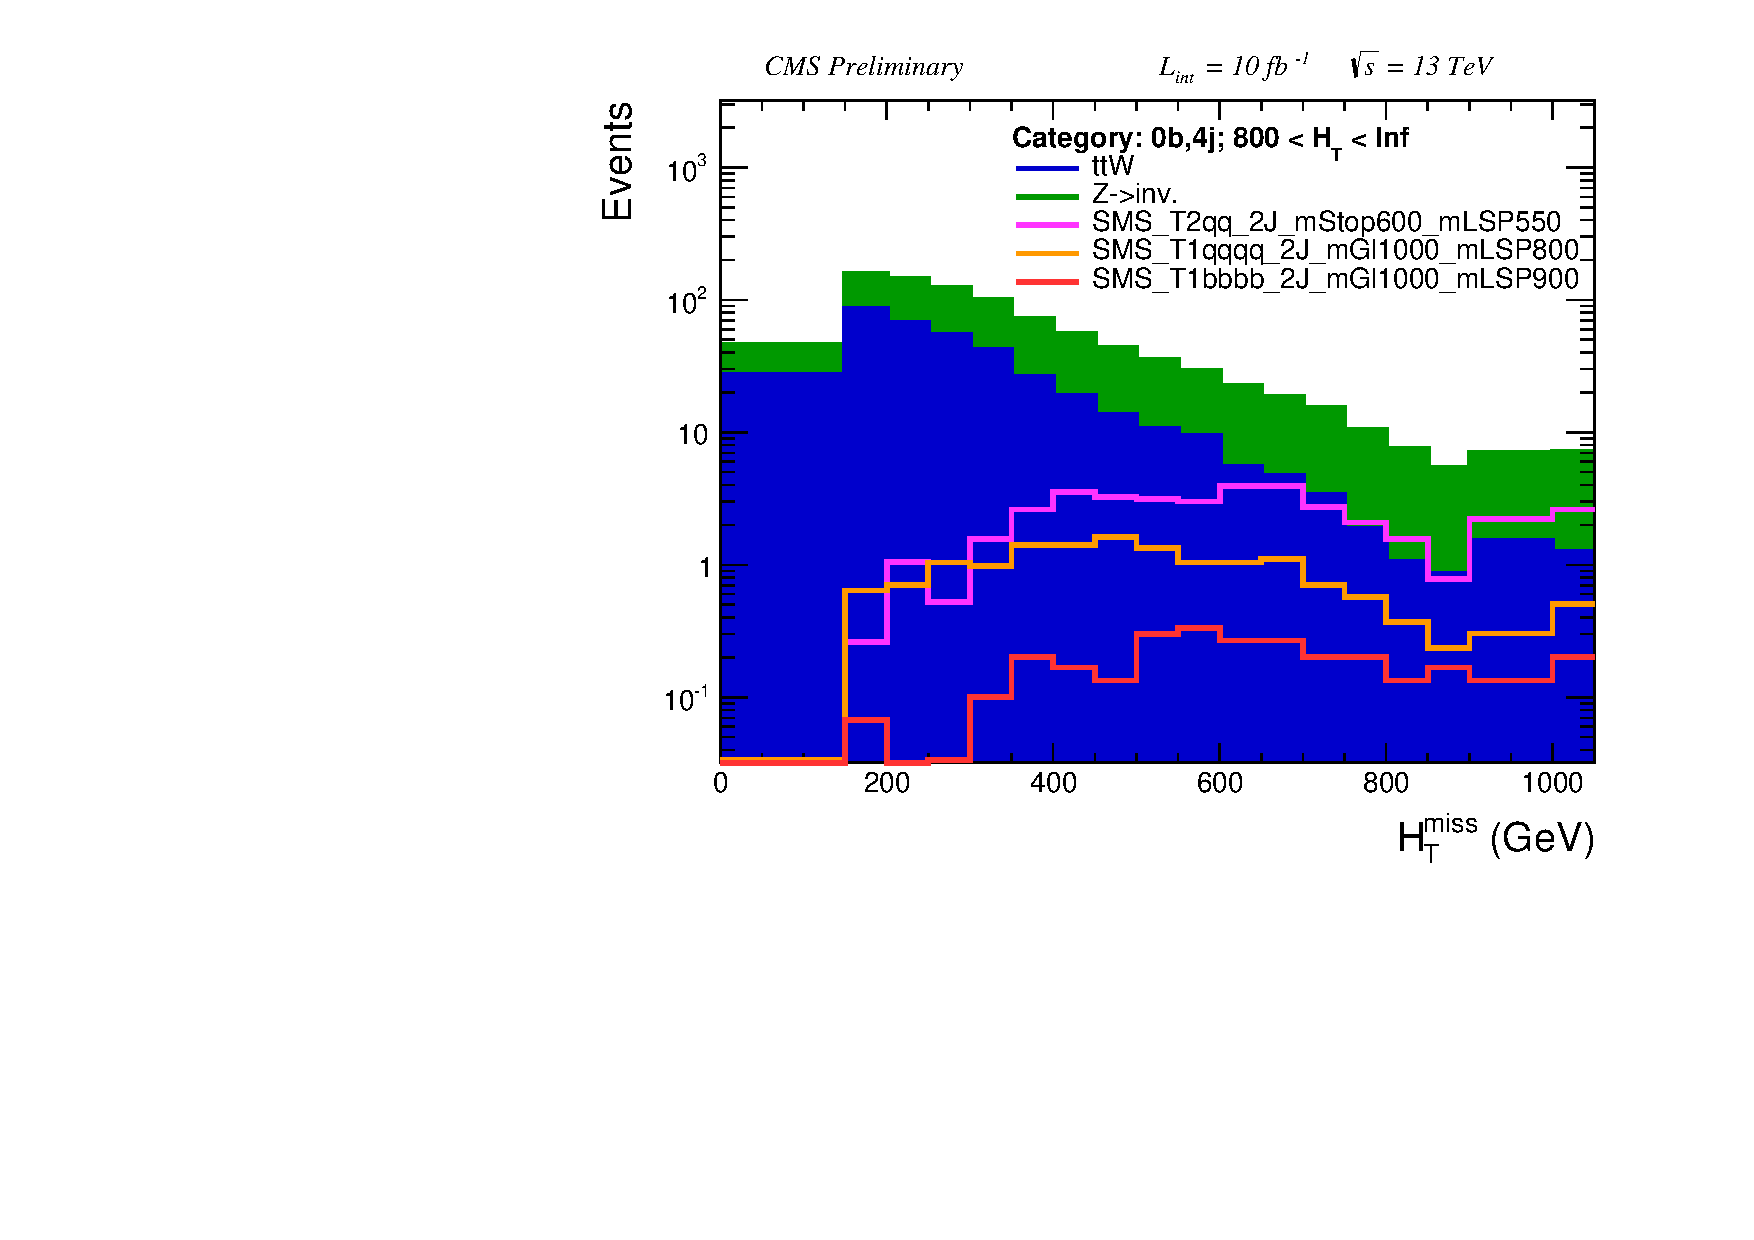
\includegraphics[width=0.5\textwidth]{figures/susyResults/MHT_eq0b_eq4j_800_Inf.pdf}} \\
    \caption{\mht templates for the $\njet=4$, $\nb=0$ category.}
    \label{fig:mht_eq0b_eq4j}
  \end{center}
\end{figure}


\begin{figure}
  \begin{center}
    \subfigure[$400 < \HT < 600  \gev$]{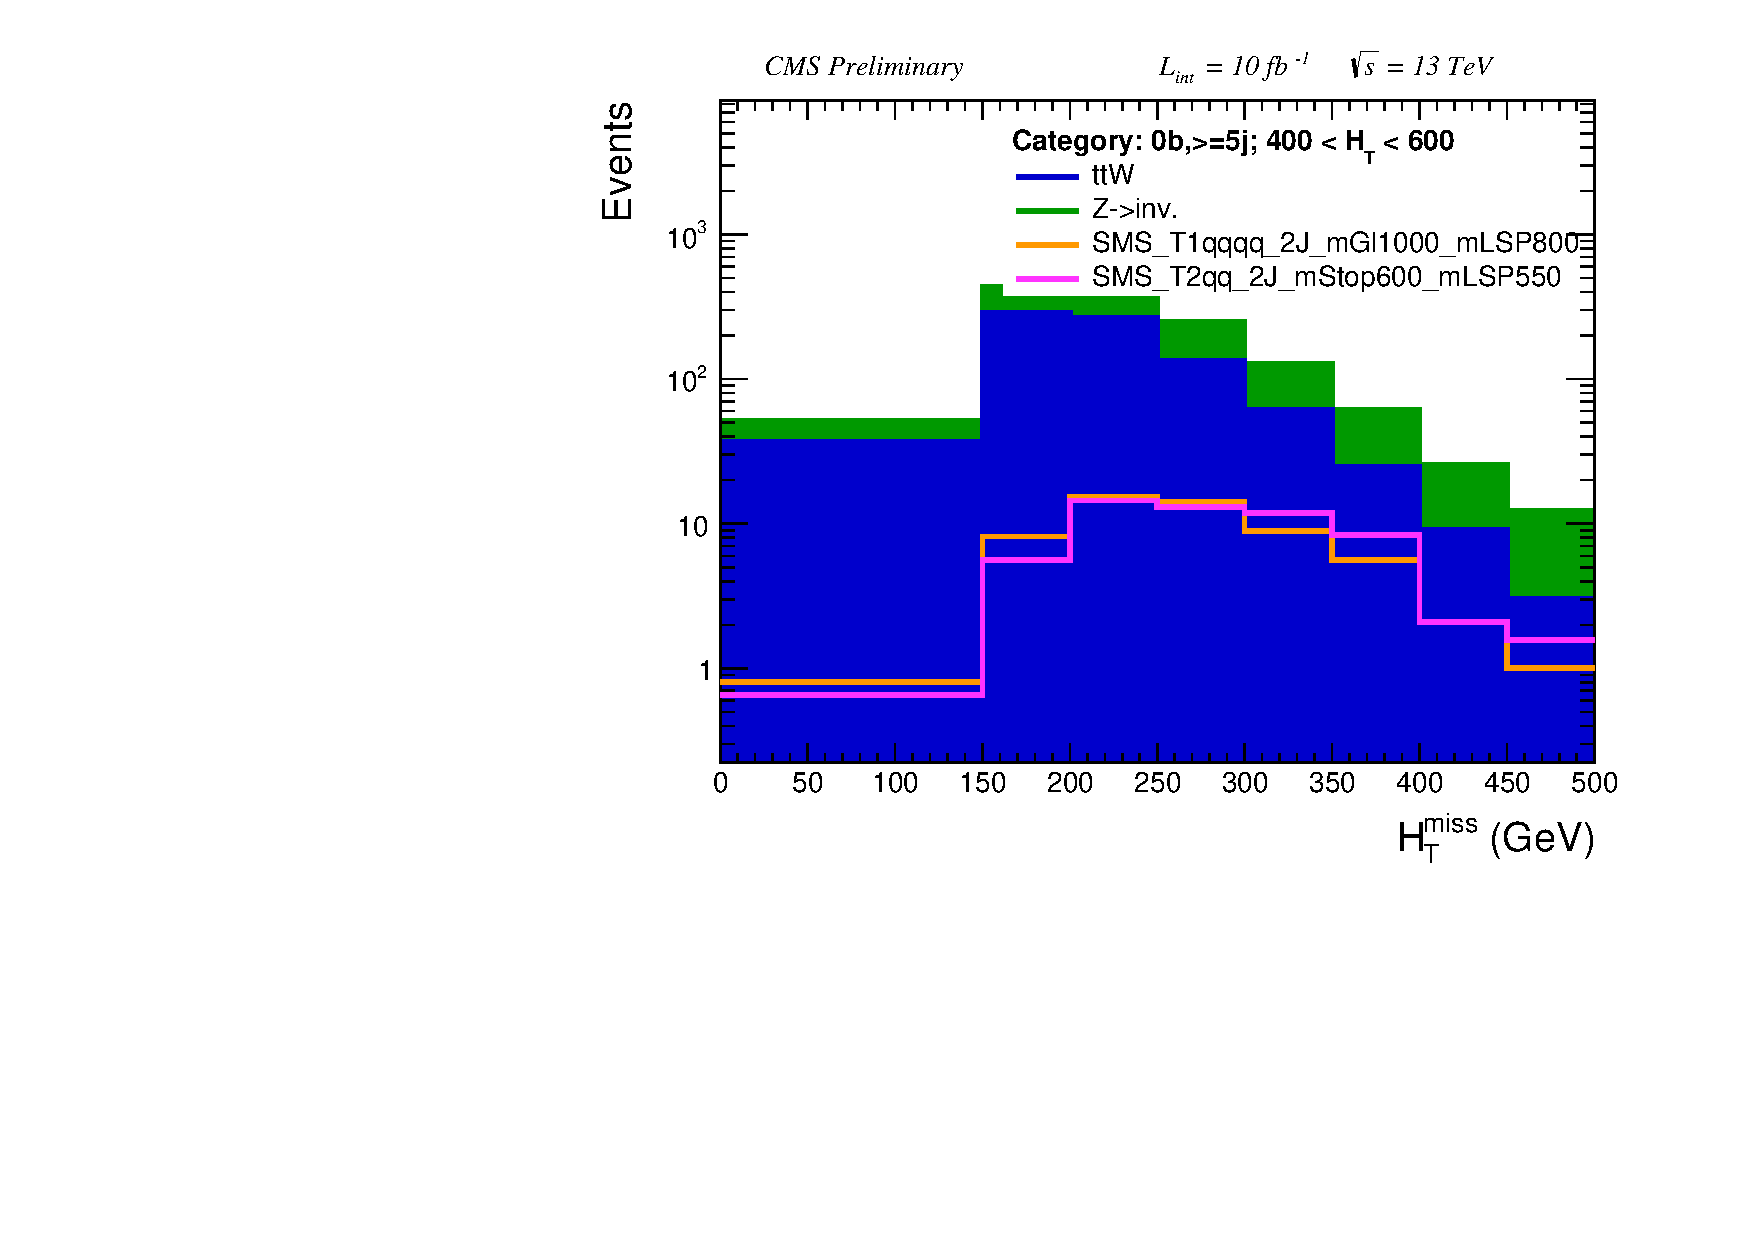
\includegraphics[width=0.5\textwidth]{figures/susyResults/MHT_eq0b_ge5j_400_600.pdf}} ~~
    \subfigure[$600 < \HT < 800  \gev$]{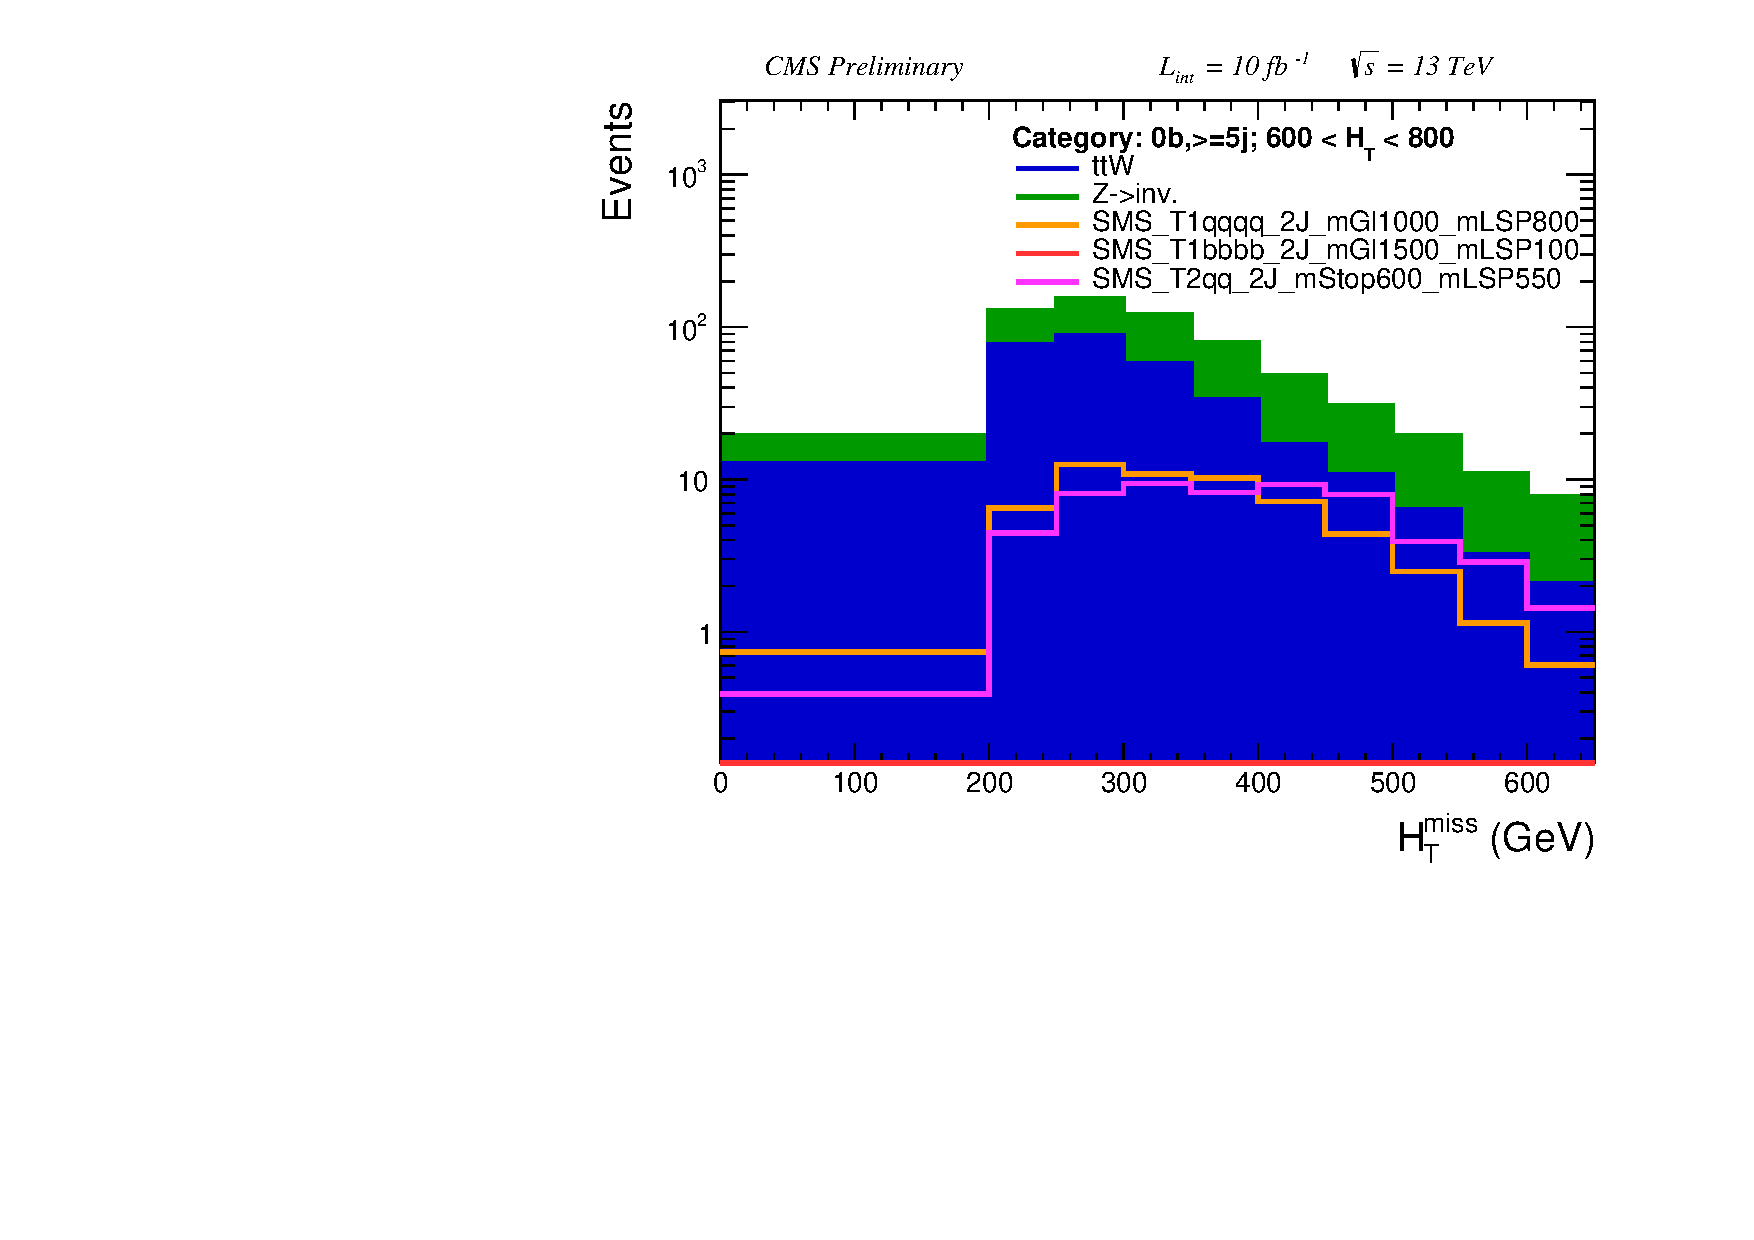
\includegraphics[width=0.5\textwidth]{figures/susyResults/MHT_eq0b_ge5j_600_800.pdf}} \\
    \subfigure[$\HT > 800 \gev$]{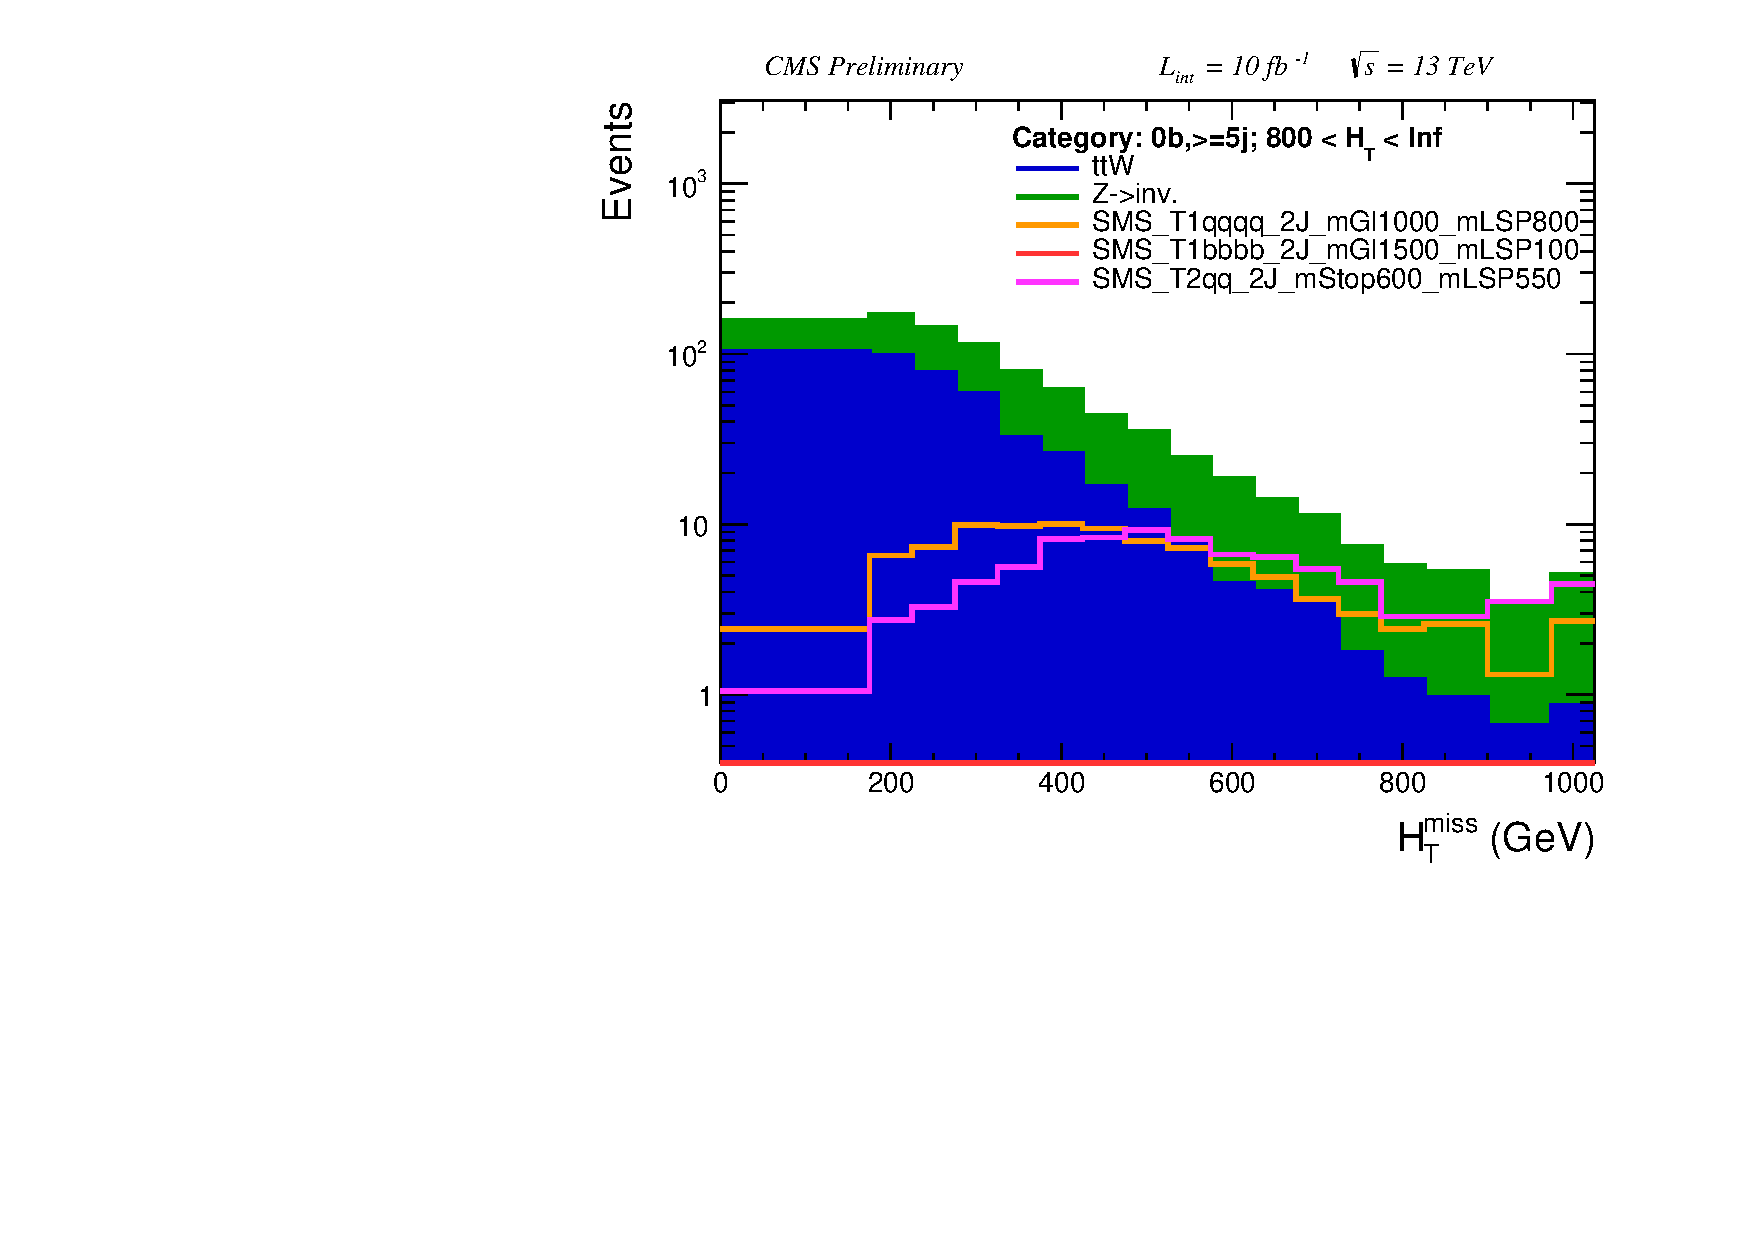
\includegraphics[width=0.5\textwidth]{figures/susyResults/MHT_eq0b_ge5j_800_Inf.pdf}}
    \caption{\mht templates for the $\njet\geq 5$, $\nb=0$ category.}
    \label{fig:mht_eq0b_ge5j}
  \end{center}
\end{figure}


\begin{figure}
  \begin{center}
    \subfigure[$350 < \HT < 400  \gev$]{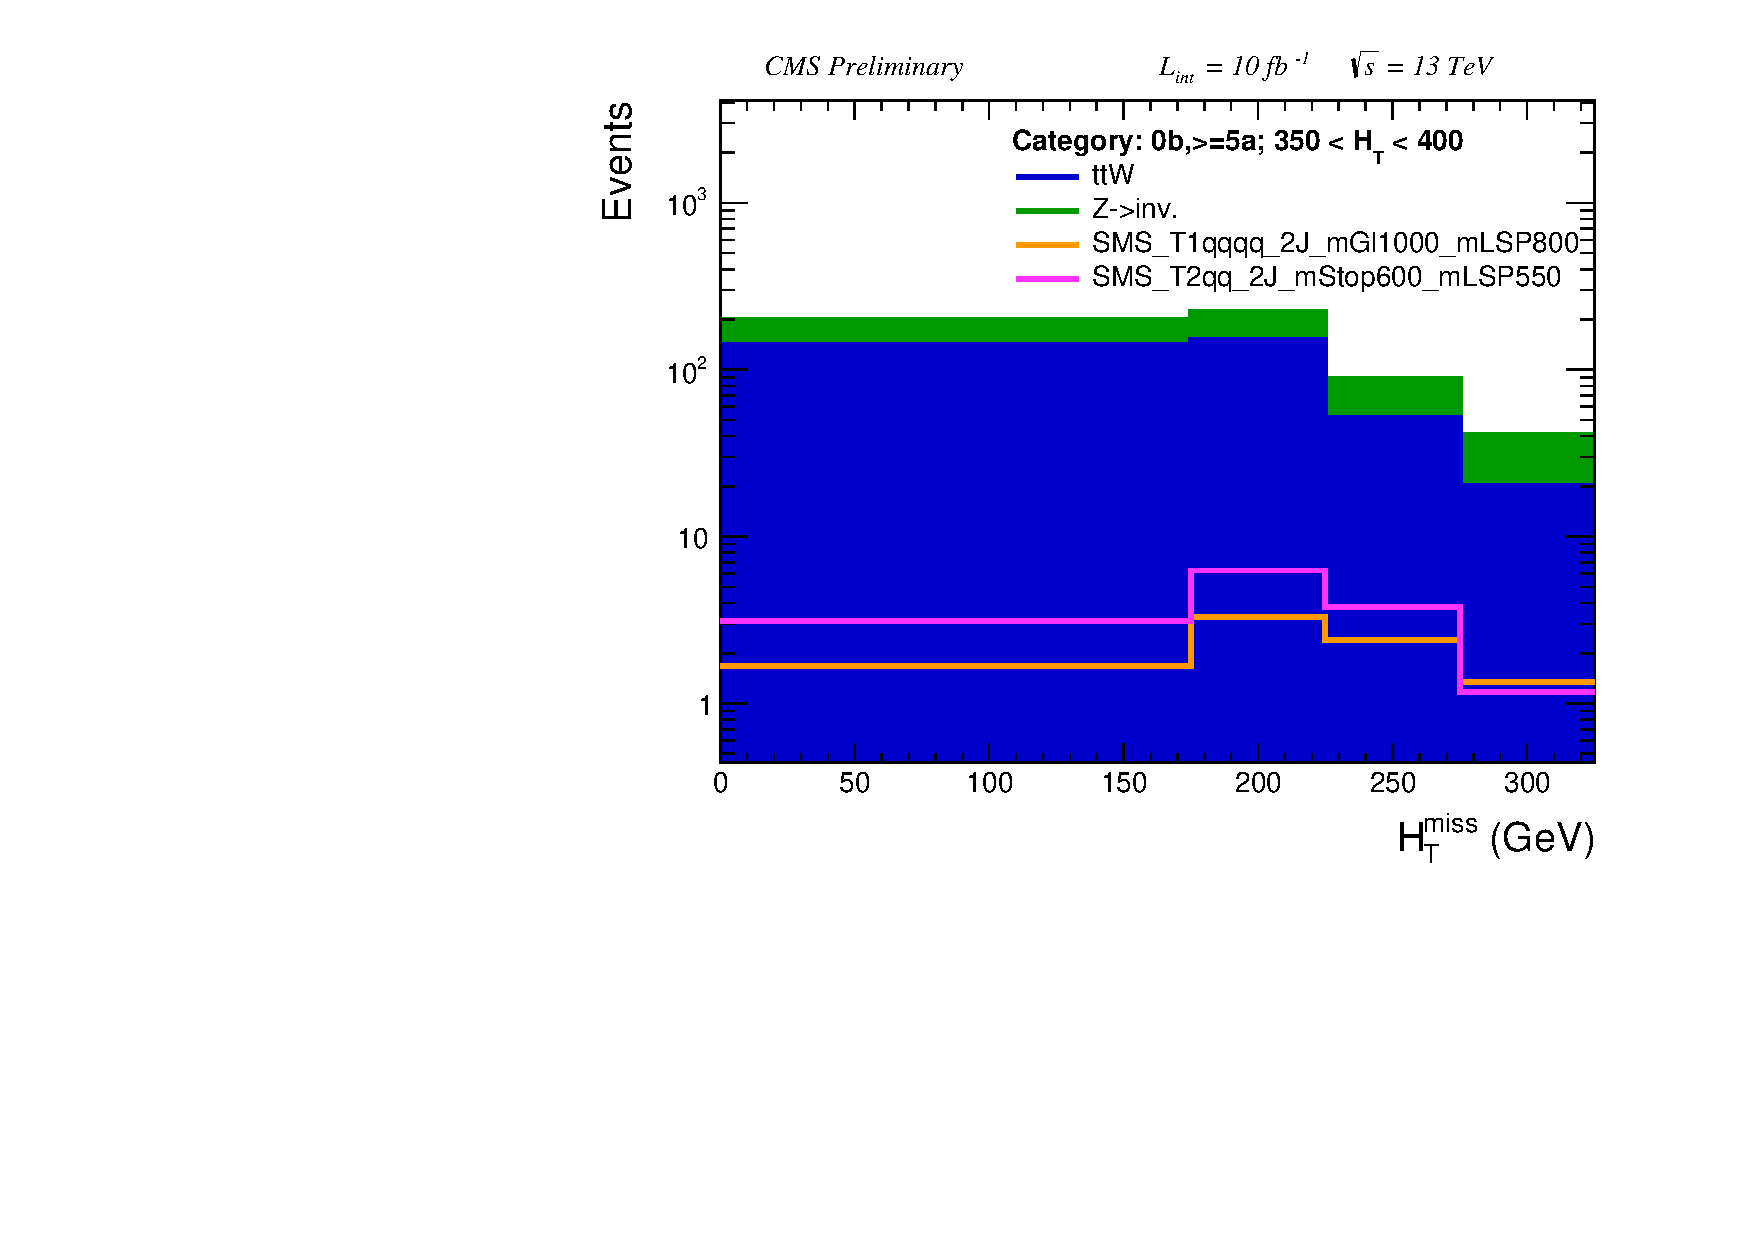
\includegraphics[width=0.5\textwidth]{figures/susyResults/MHT_eq0b_ge5a_350_400.pdf}} ~~
    \subfigure[$400 < \HT < 600  \gev$]{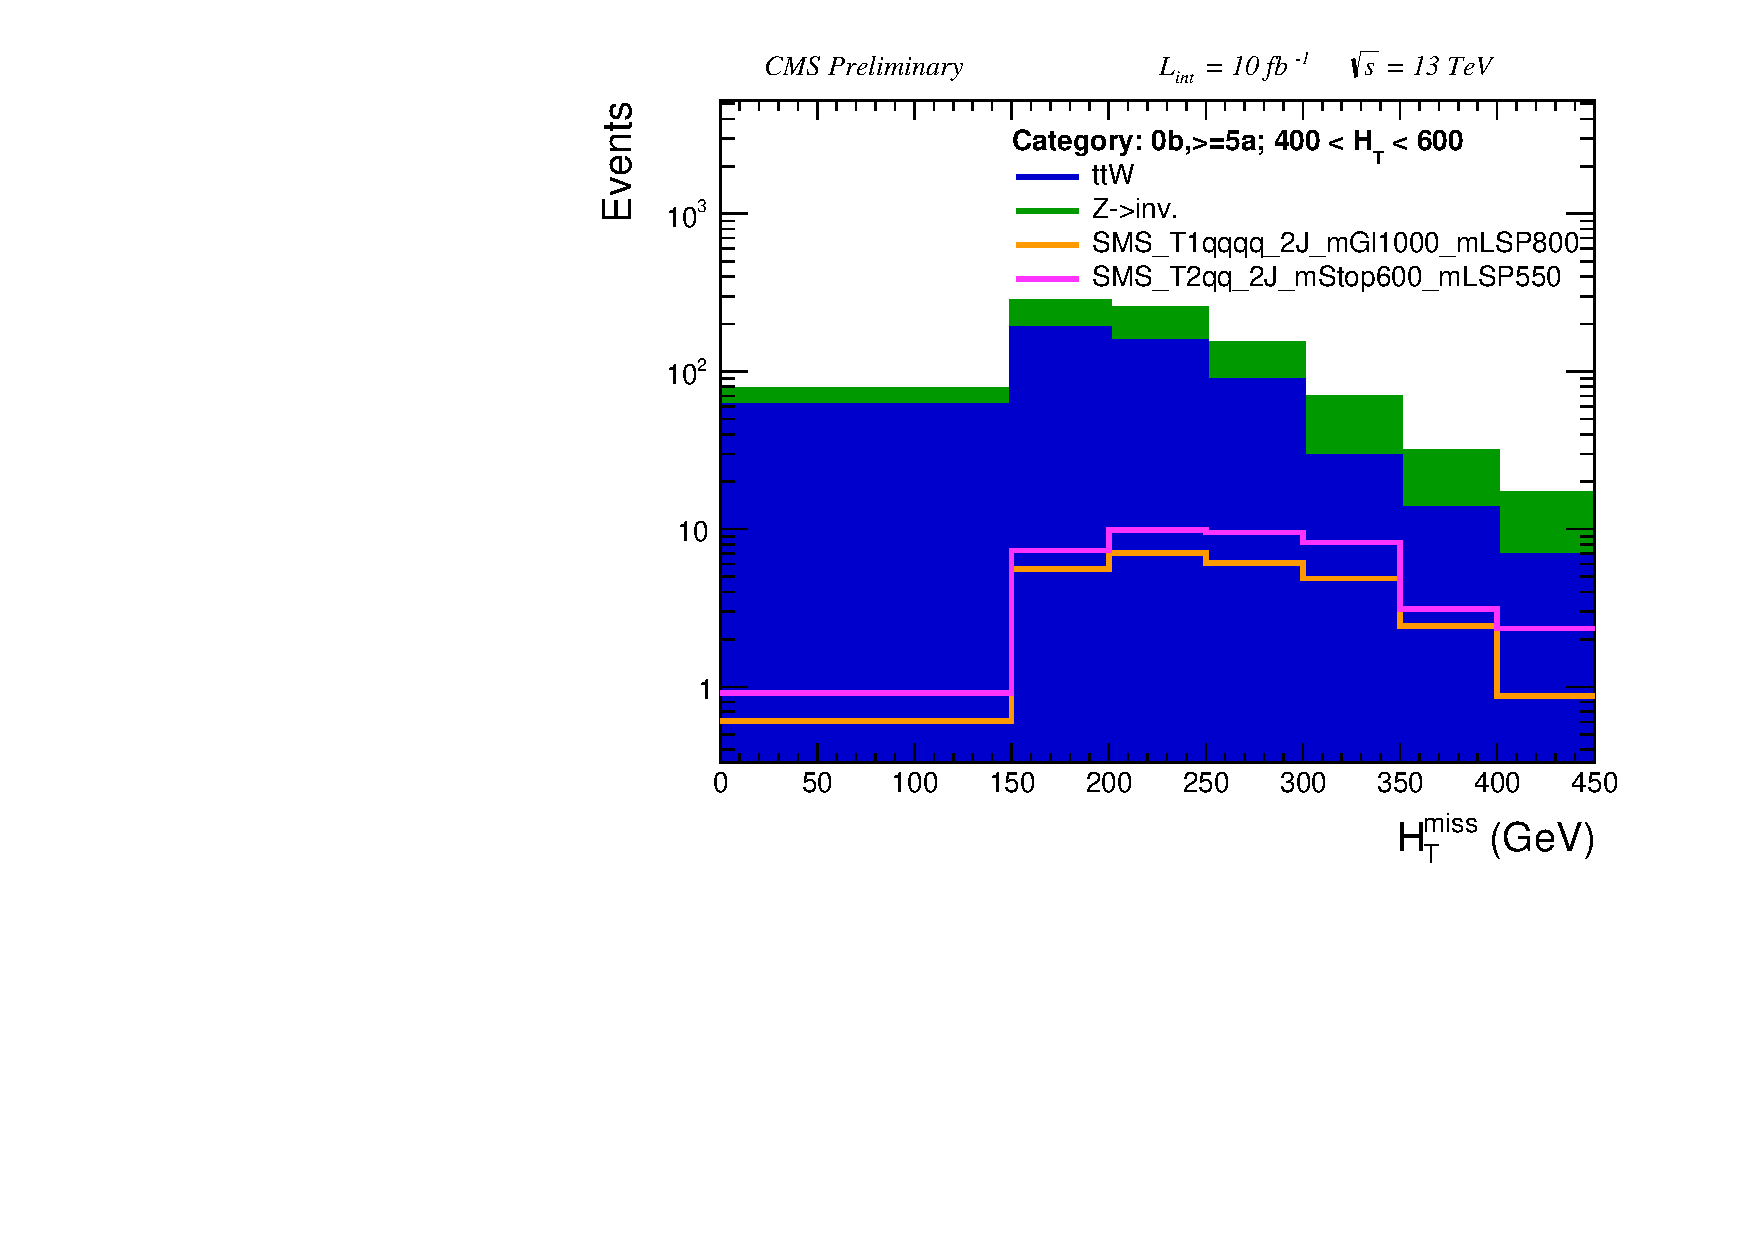
\includegraphics[width=0.5\textwidth]{figures/susyResults/MHT_eq0b_ge5a_400_600.pdf}}
    \caption{\mht templates for the $\njet\geq 5$ (asymmetric), $\nb=0$ category.}
    \label{fig:mht_eq0b_ge5a}
  \end{center}
\end{figure}


\begin{figure}
  \begin{center}
    \subfigure[$400 < \HT < 600  \gev$]{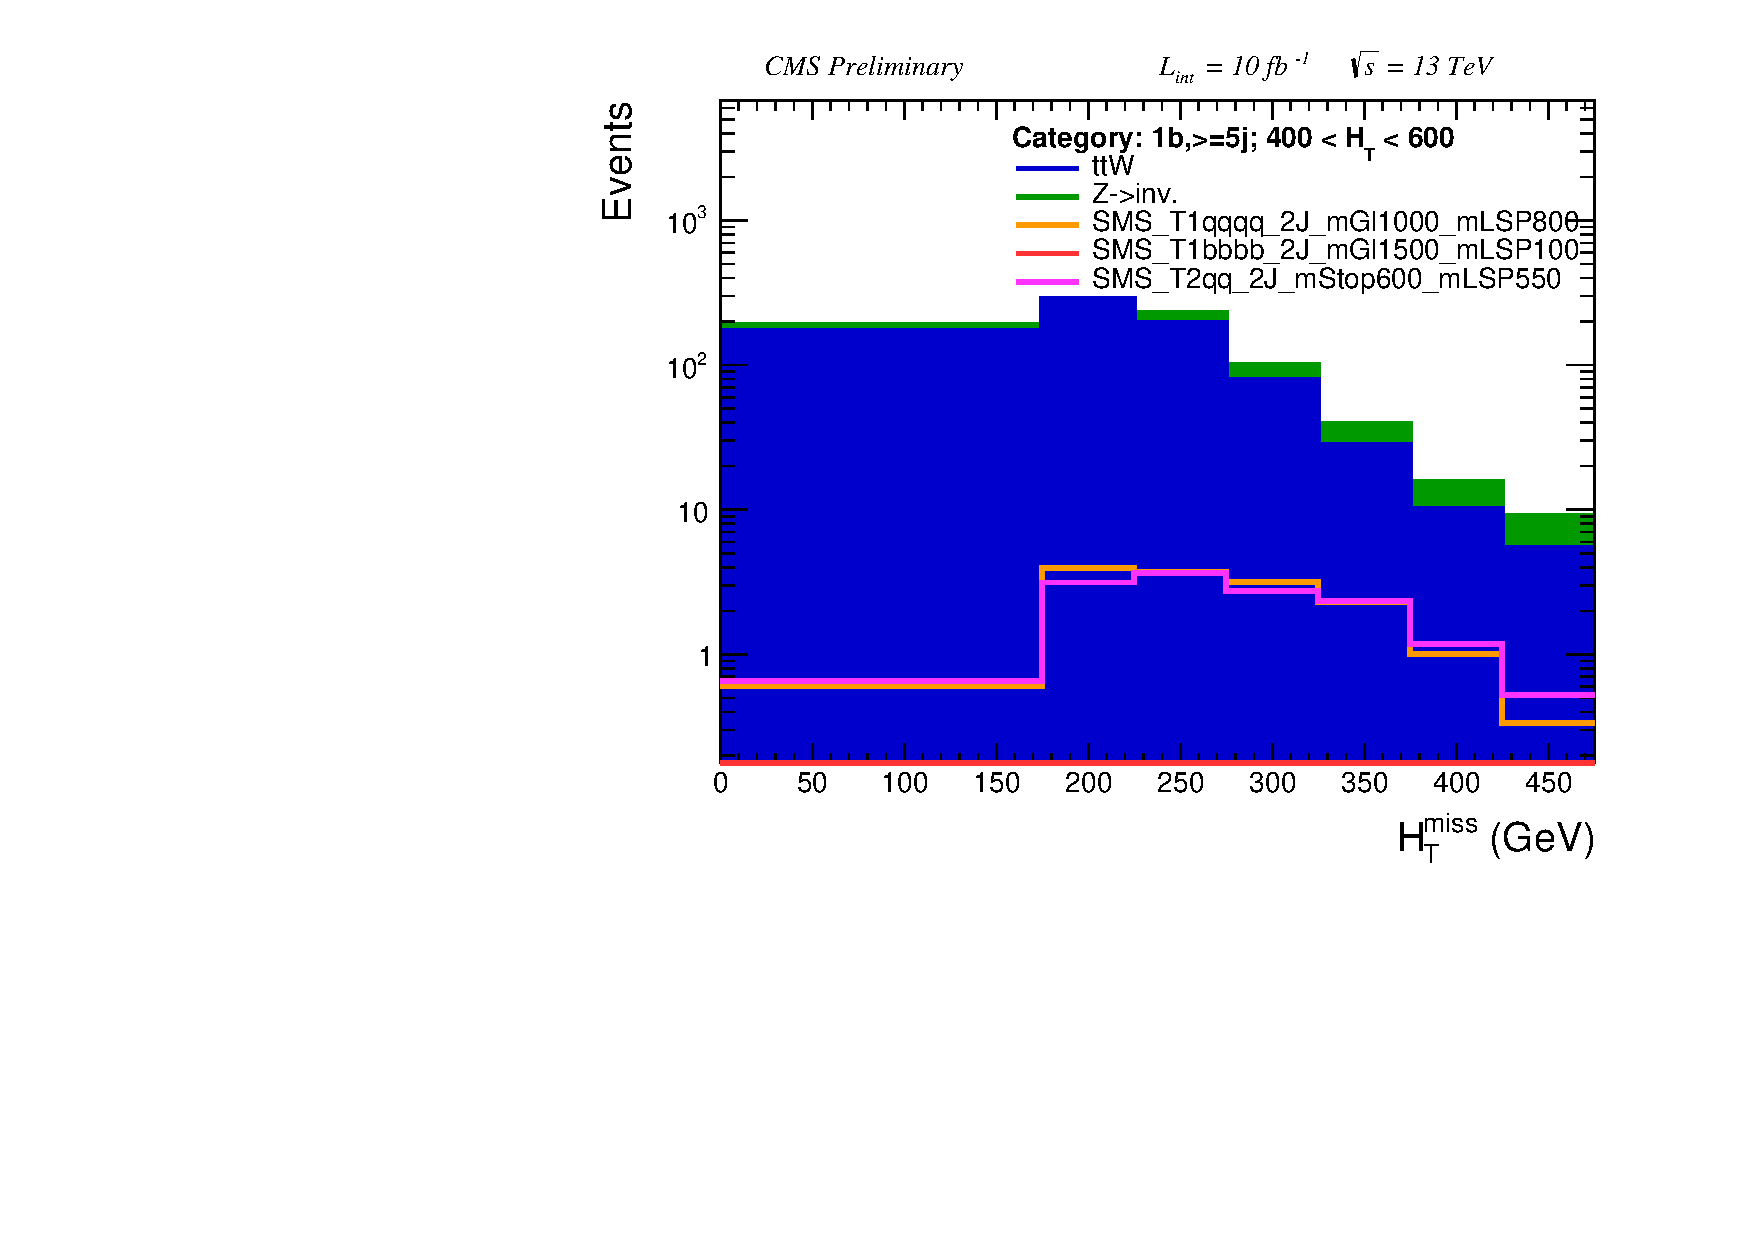
\includegraphics[width=0.5\textwidth]{figures/susyResults/MHT_eq1b_ge5j_400_600.pdf}} ~~
    \subfigure[$600 < \HT < 800  \gev$]{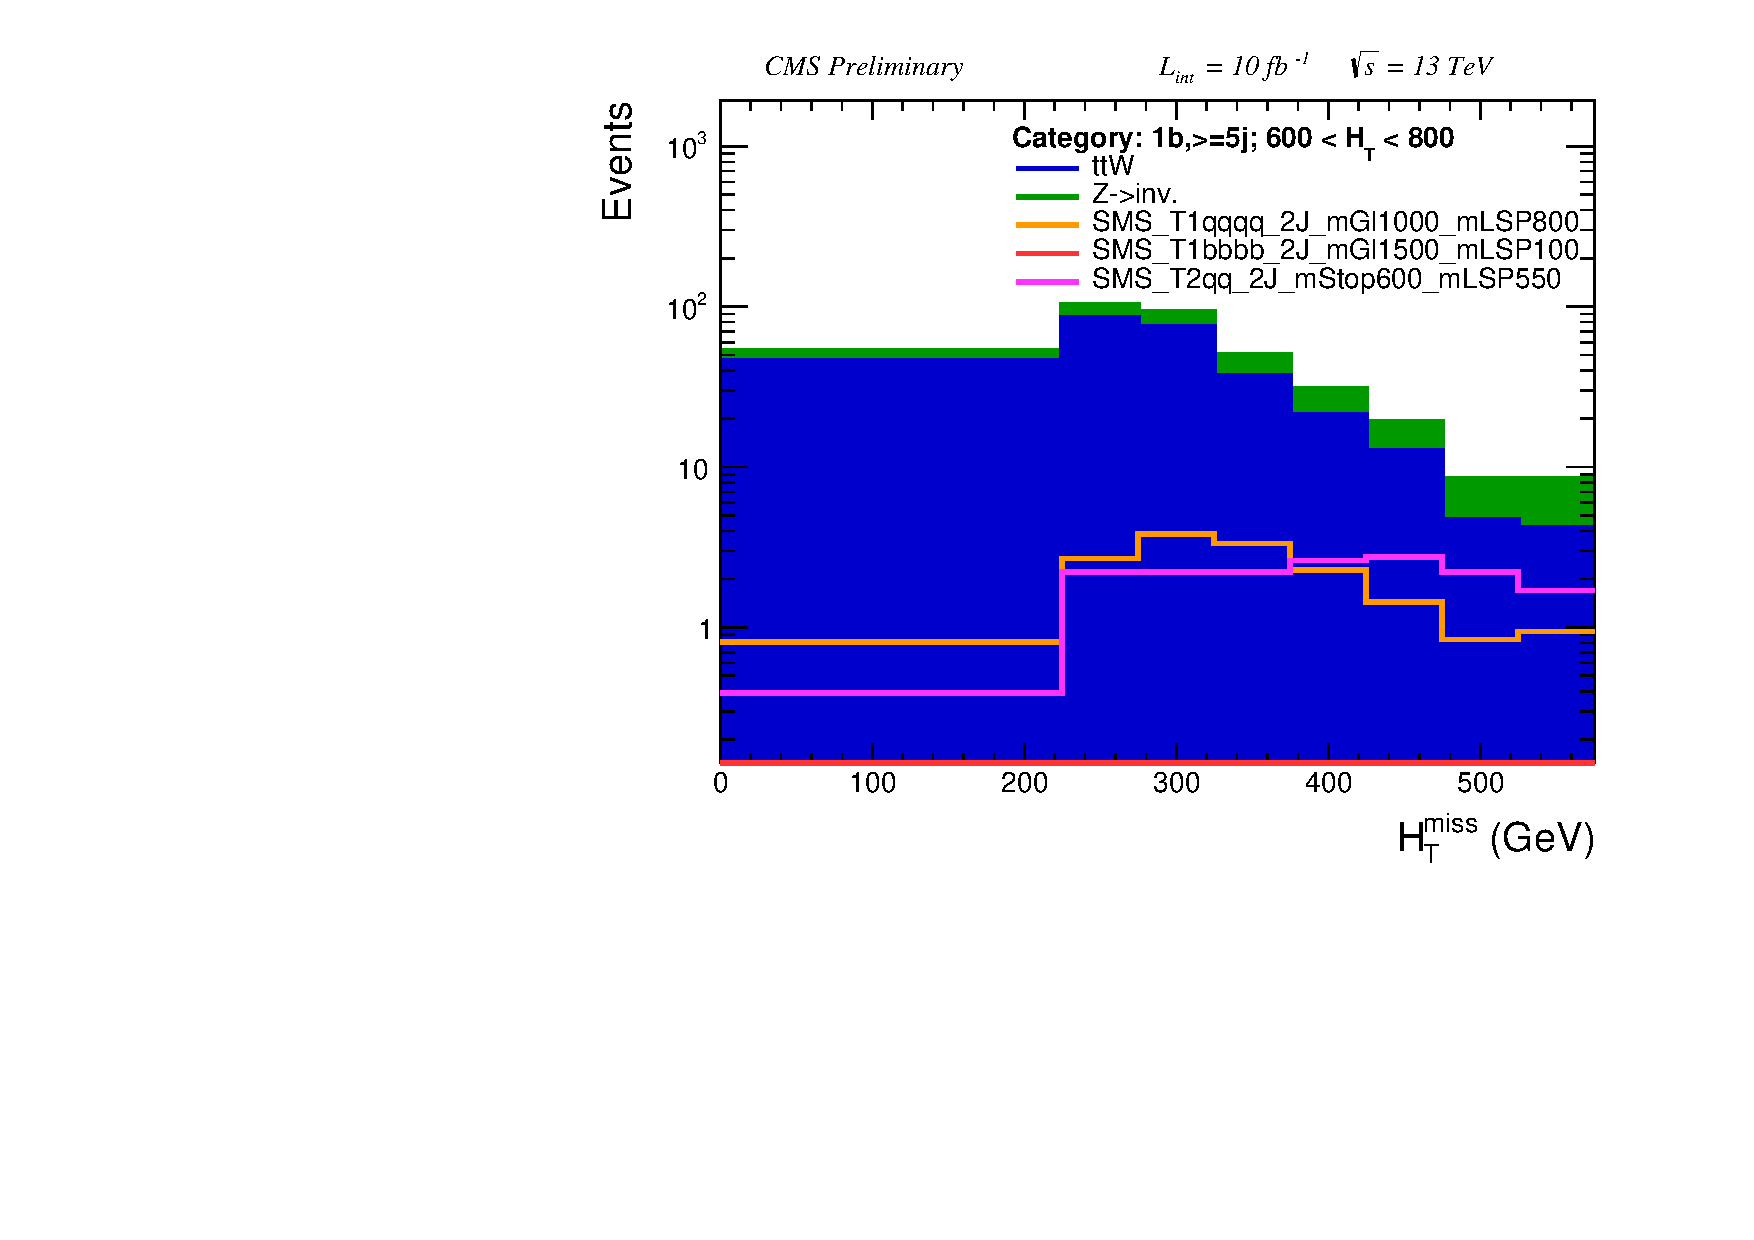
\includegraphics[width=0.5\textwidth]{figures/susyResults/MHT_eq1b_ge5j_600_800.pdf}} \\
    \subfigure[$\HT > 800 \gev$]{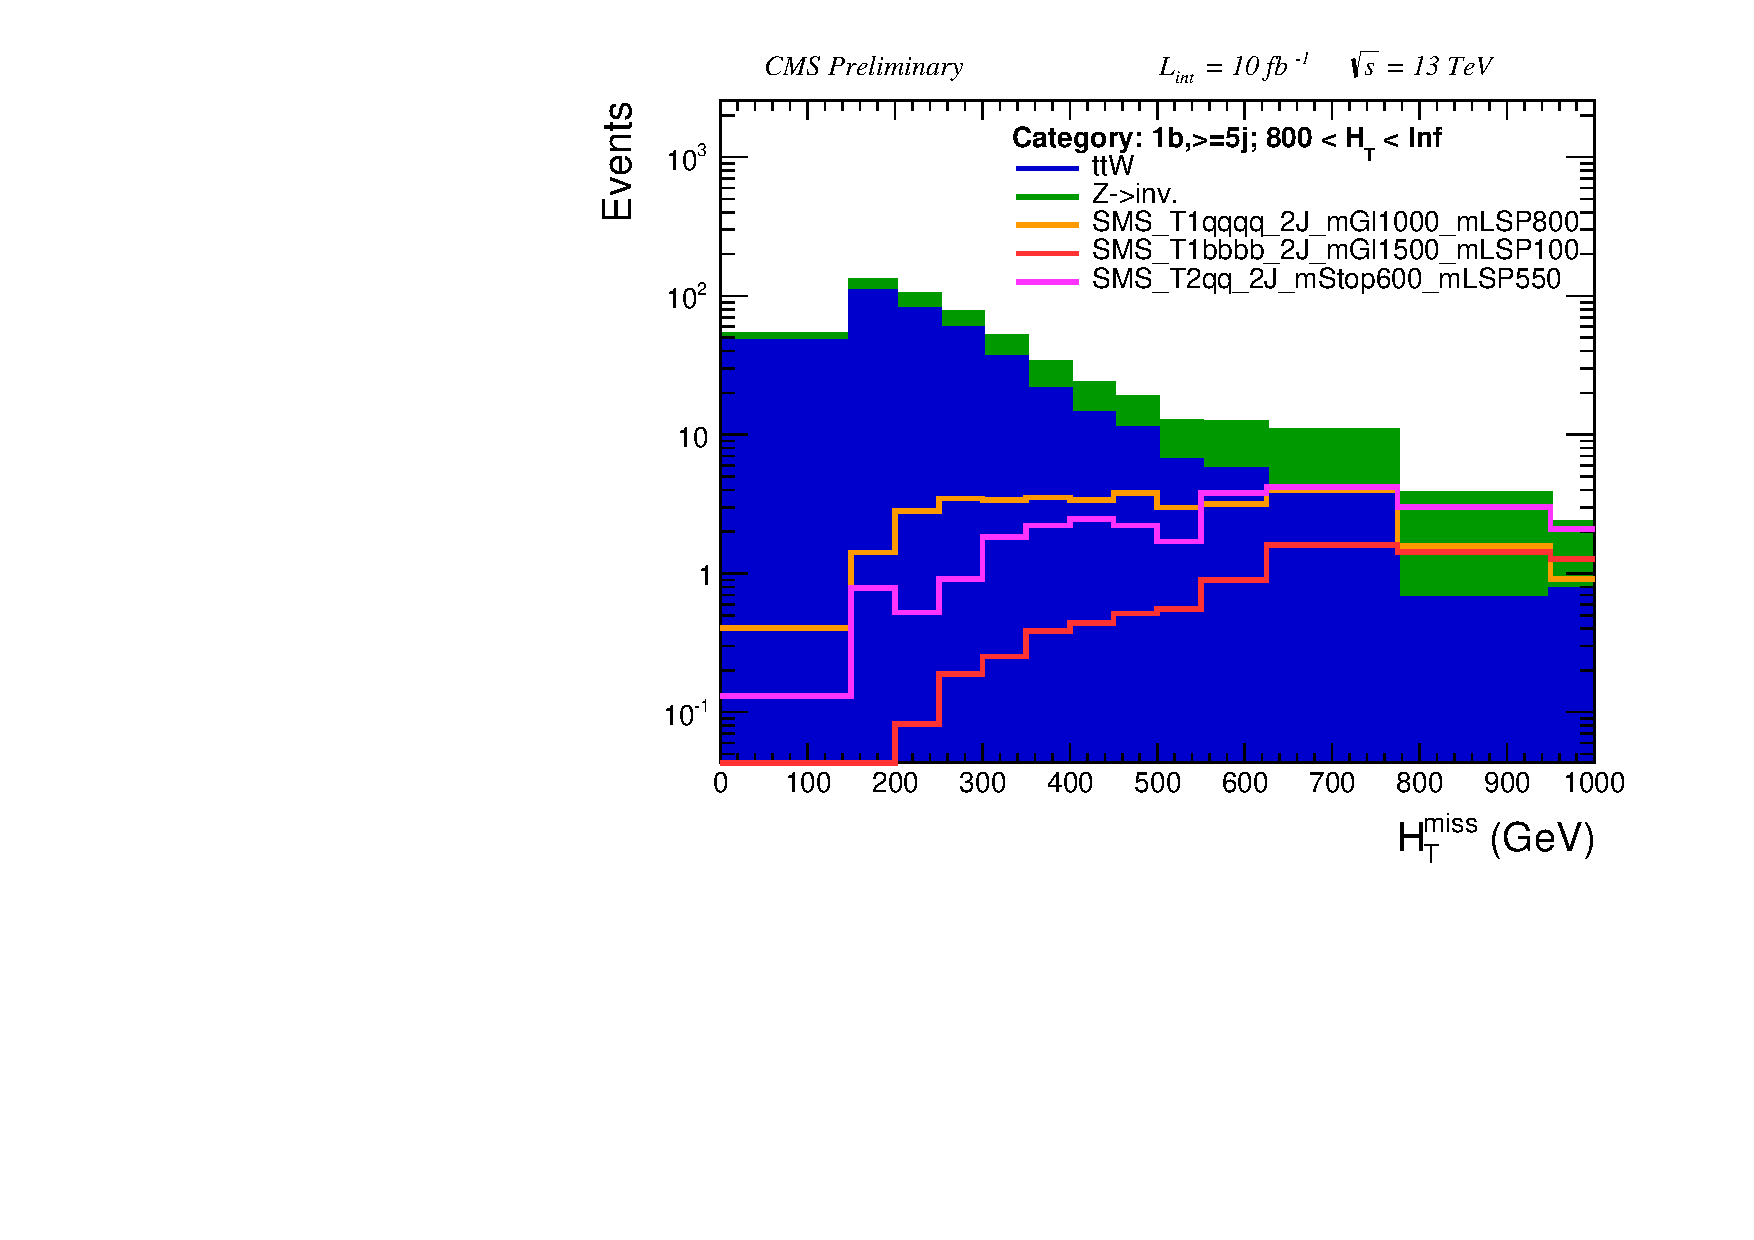
\includegraphics[width=0.5\textwidth]{figures/susyResults/MHT_eq1b_ge5j_800_Inf.pdf}}
    \caption{\mht templates for the $\njet\geq 5$, $\nb=1$ category.}
    \label{fig:mht_eq1b_ge5j}
  \end{center}
\end{figure}


\begin{figure}
  \begin{center}
    \subfigure[$350 < \HT < 400  \gev$]{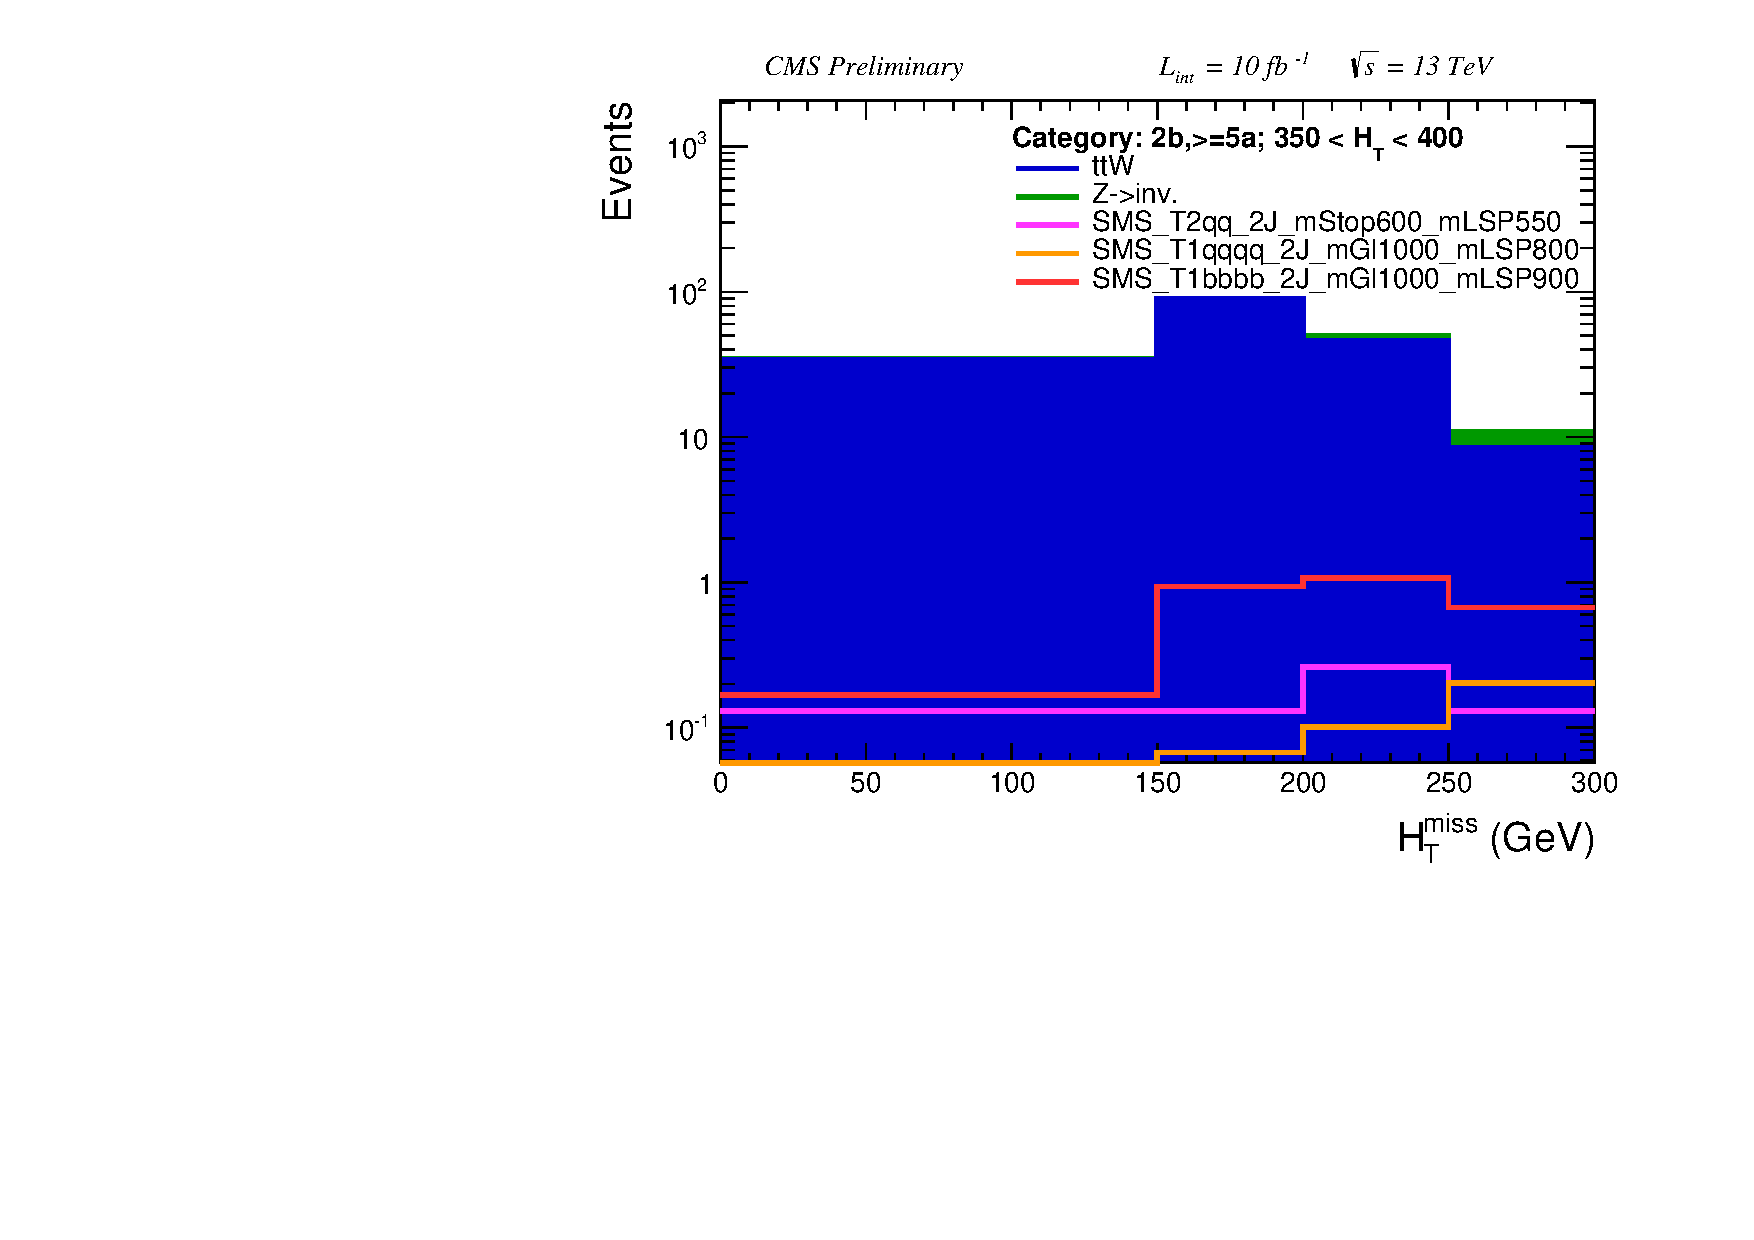
\includegraphics[width=0.5\textwidth]{figures/susyResults/MHT_eq2b_ge5a_350_400.pdf}} ~~
    \subfigure[$400 < \HT < 600  \gev$]{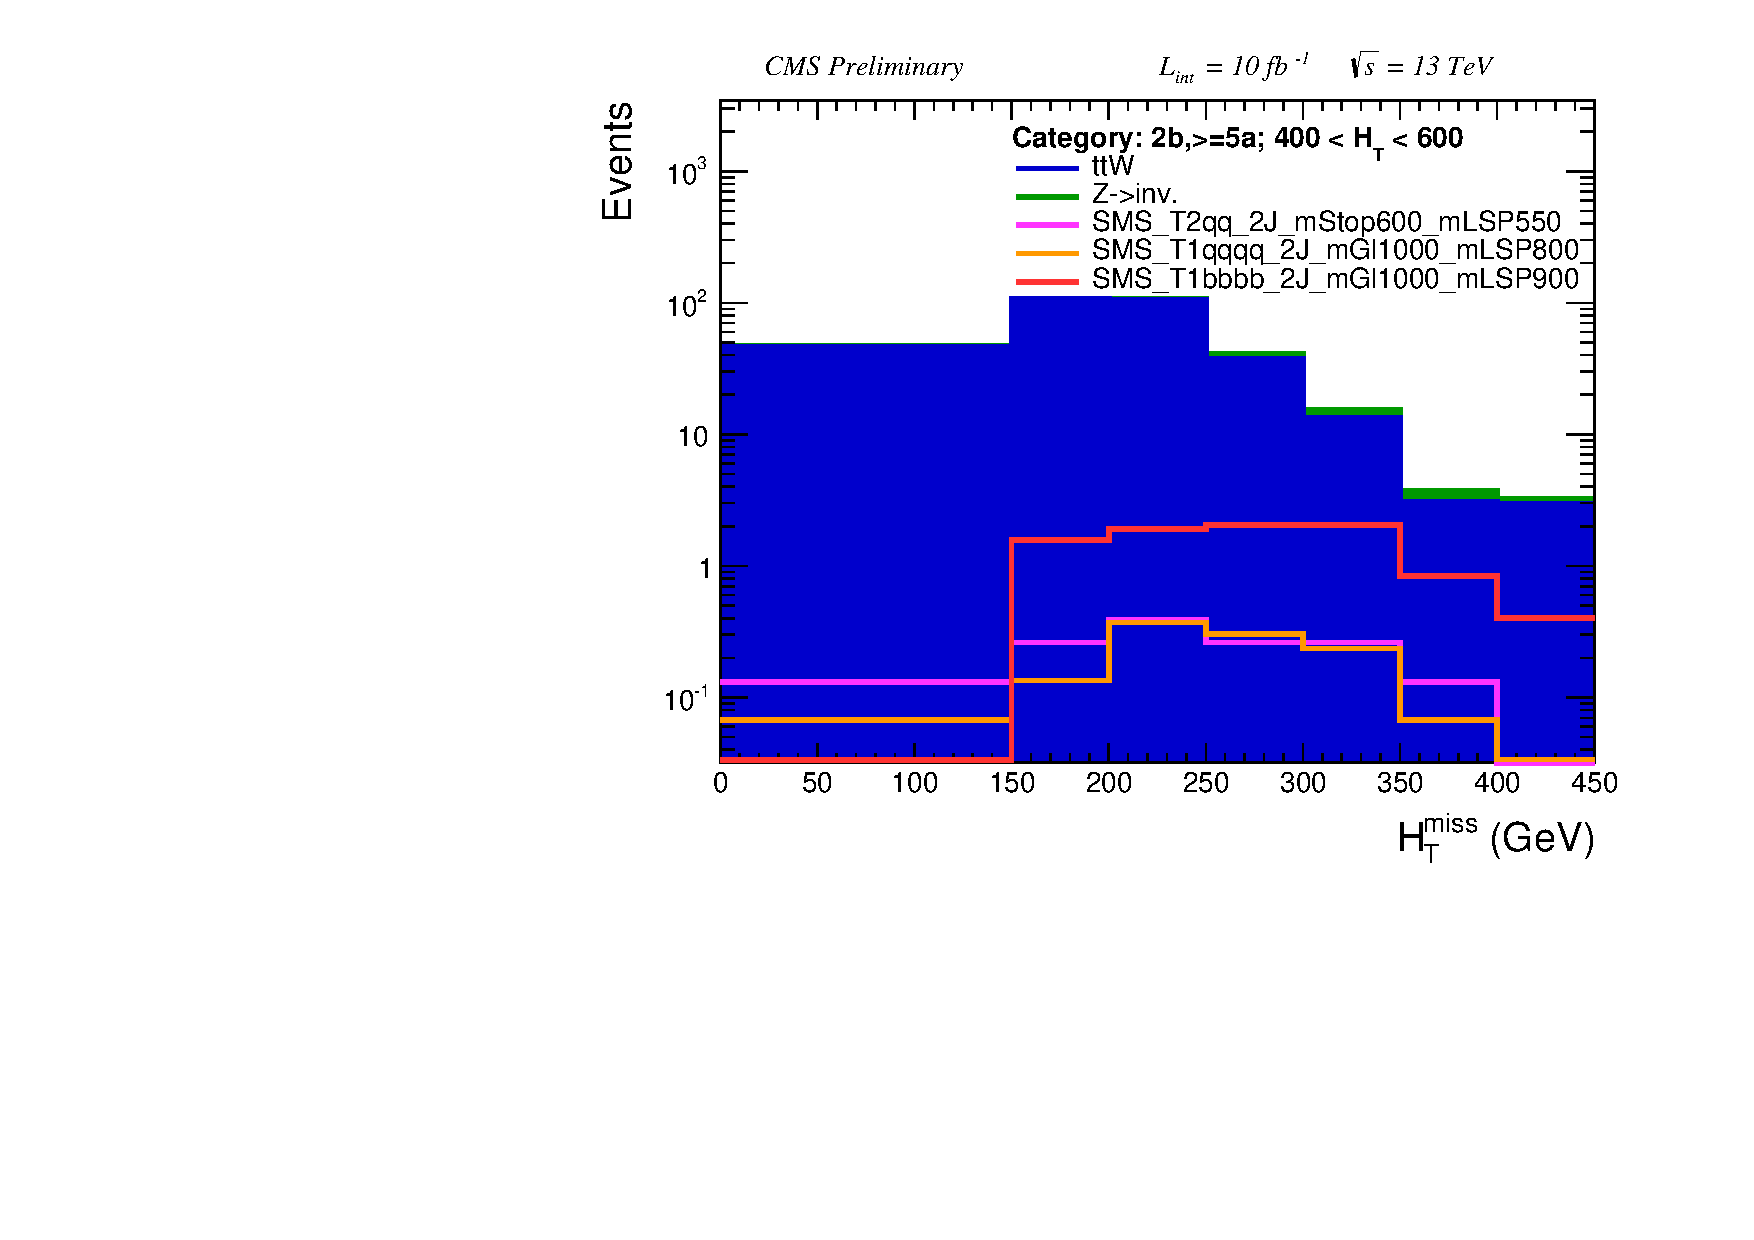
\includegraphics[width=0.5\textwidth]{figures/susyResults/MHT_eq2b_ge5a_400_600.pdf}} \\
    \subfigure[$600 < \HT < 800  \gev$]{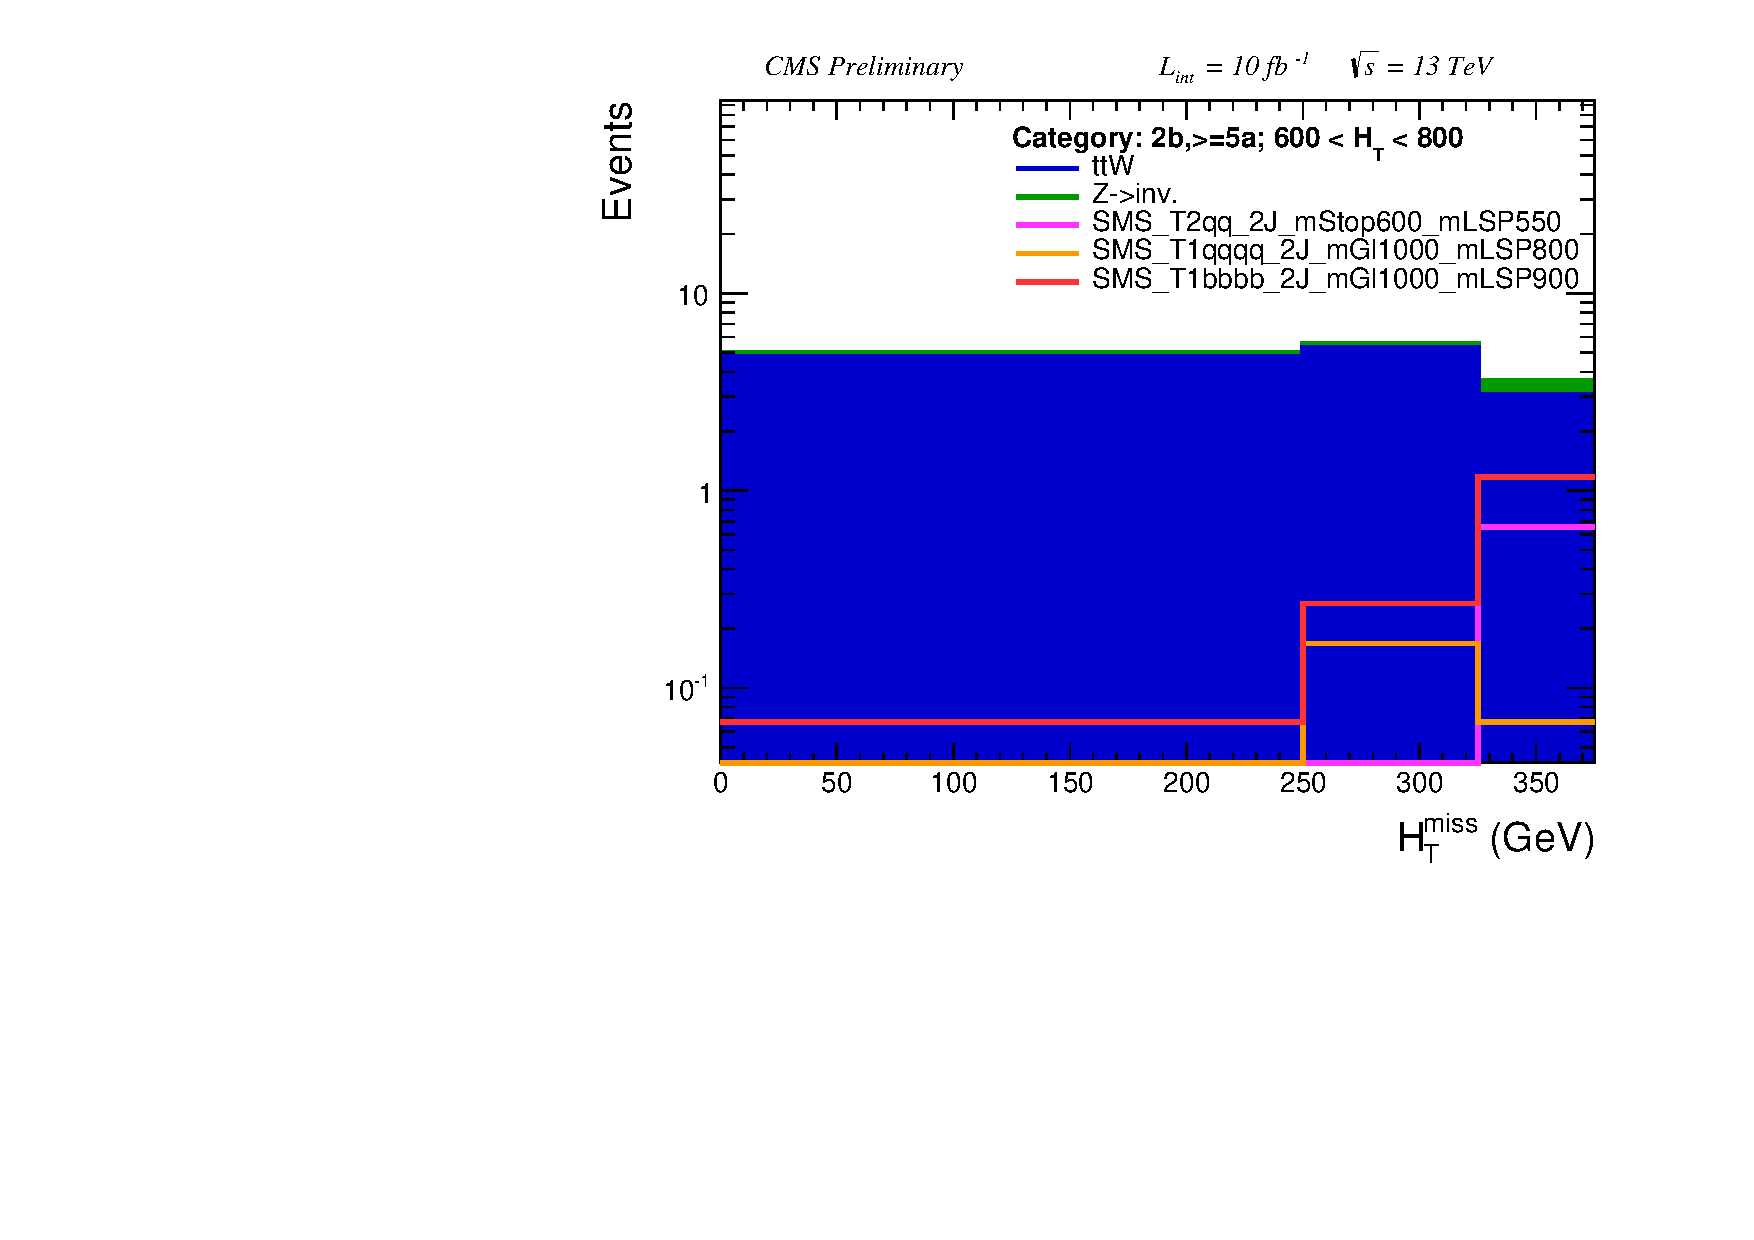
\includegraphics[width=0.5\textwidth]{figures/susyResults/MHT_eq2b_ge5a_600_800.pdf}} ~~
    \subfigure[$\HT > 800  \gev$]{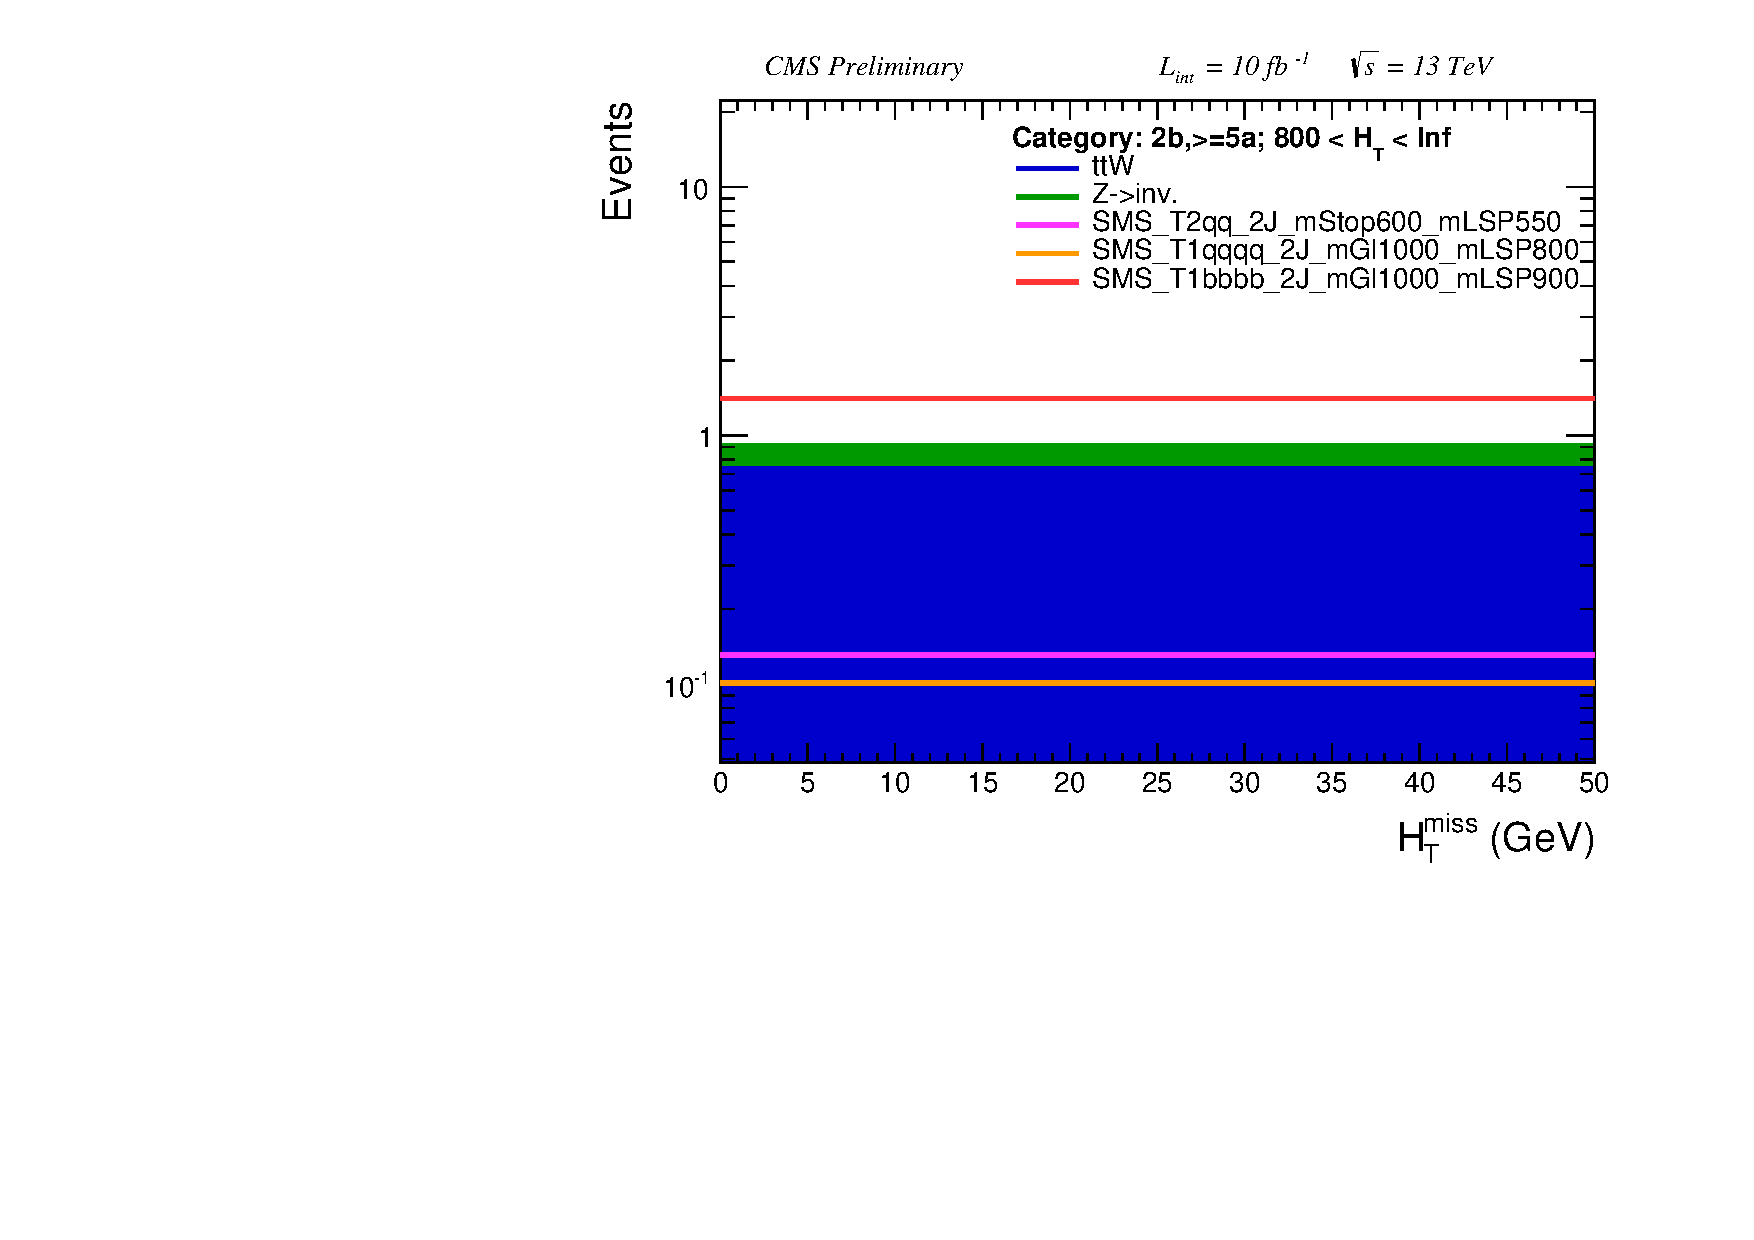
\includegraphics[width=0.5\textwidth]{figures/susyResults/MHT_eq2b_ge5a_800_Inf.pdf}} \\
    \caption{\mht templates for the $\njet=5$ (asymmetric), $\nb=2$ category.}
    \label{fig:mht_eq2b_ge5a}
  \end{center}
\end{figure}


\begin{figure}
  \begin{center}
    \subfigure[$400 < \HT < 600  \gev$]{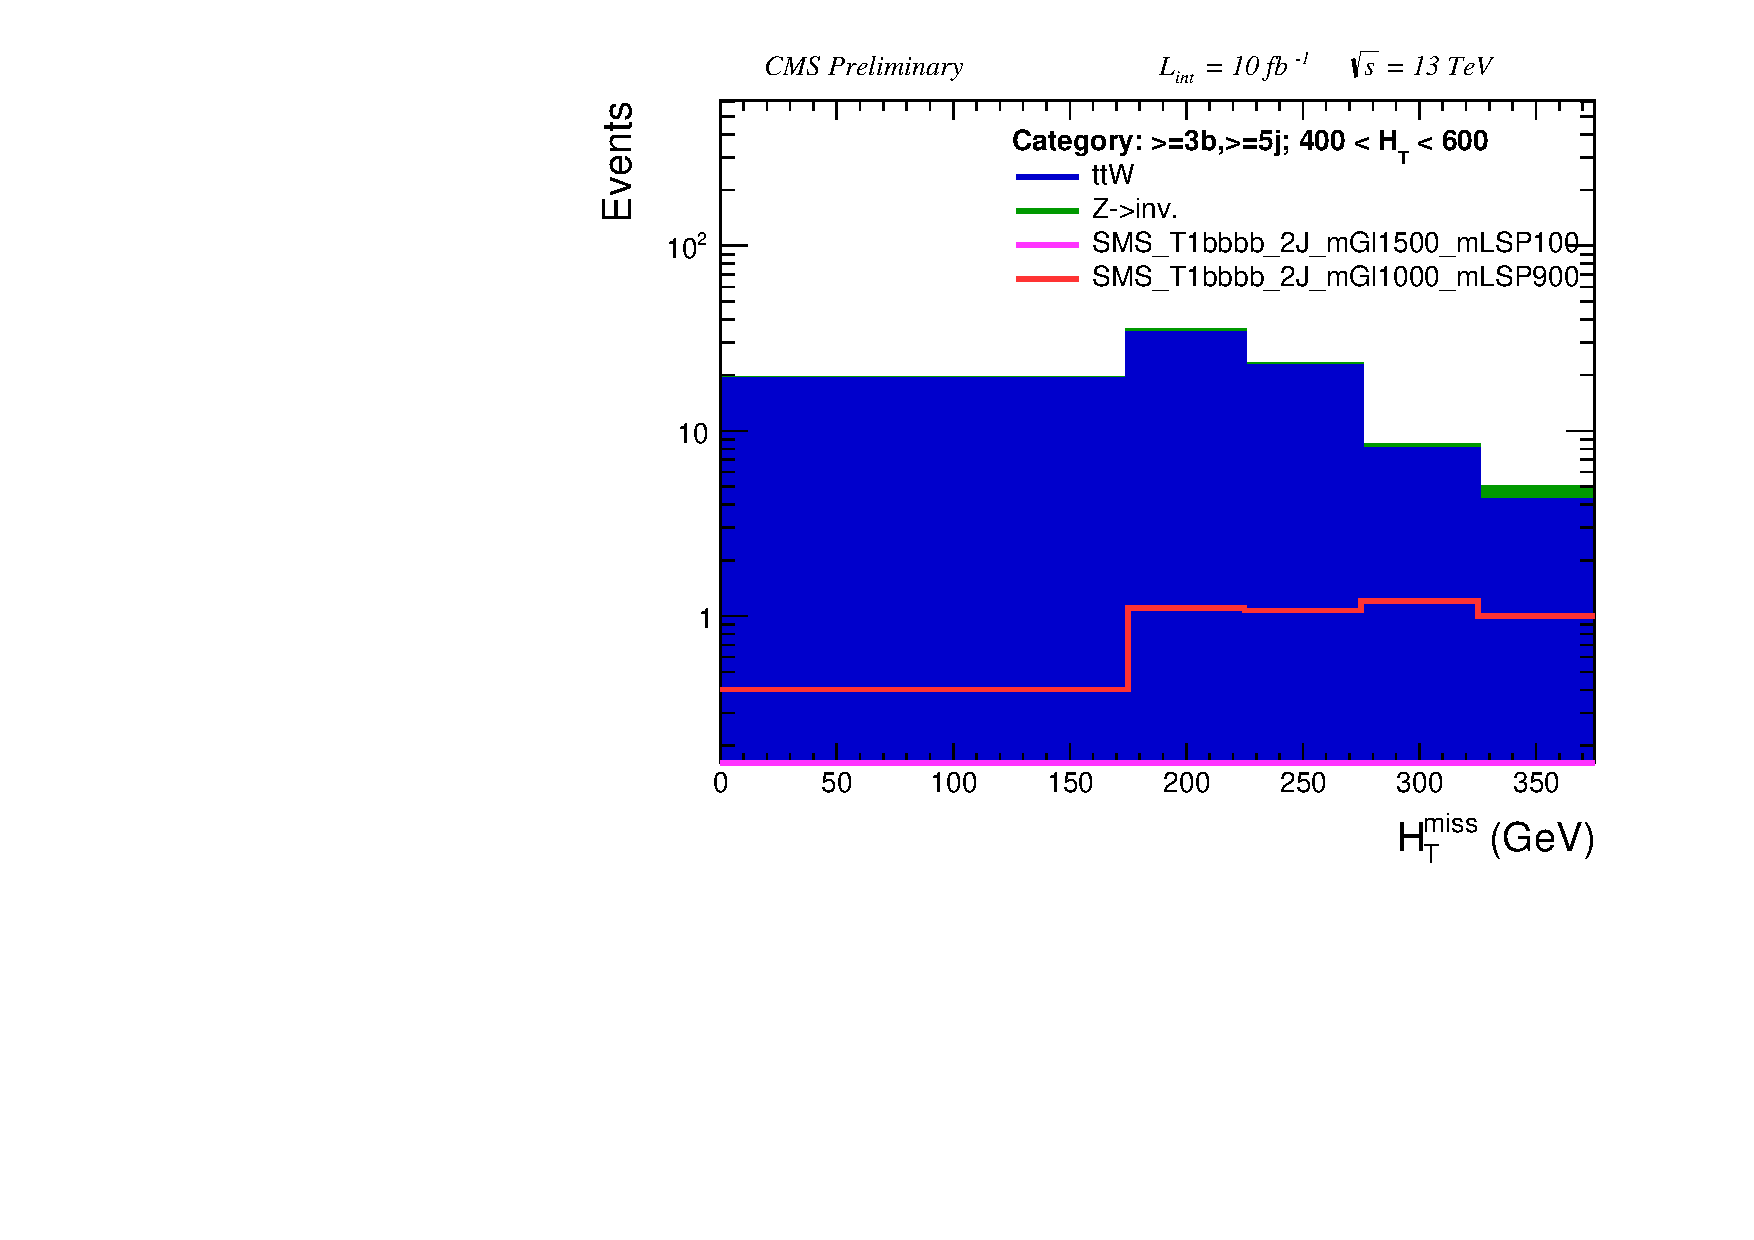
\includegraphics[width=0.5\textwidth]{figures/susyResults/MHT_ge3b_ge5j_400_600.pdf}} ~~
    \subfigure[$600 < \HT < 800  \gev$]{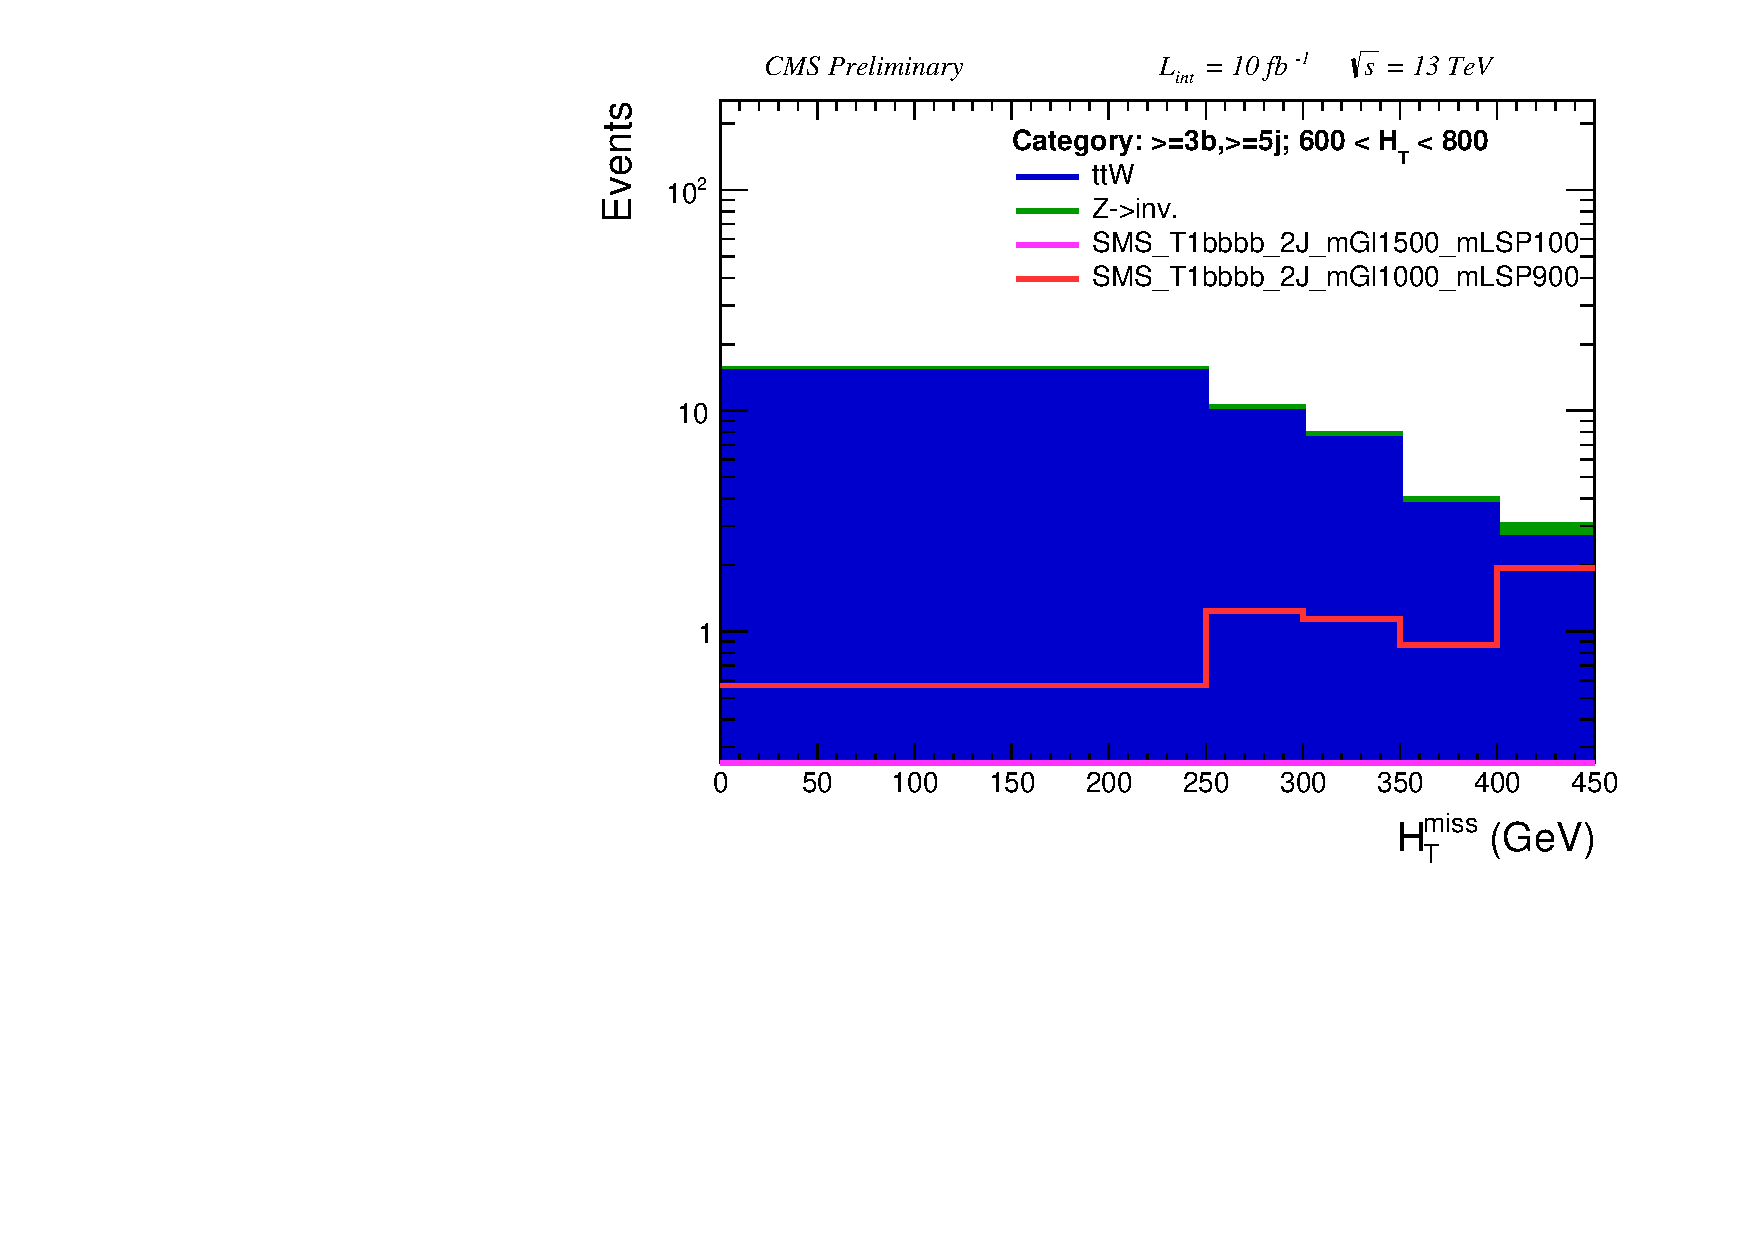
\includegraphics[width=0.5\textwidth]{figures/susyResults/MHT_ge3b_ge5j_600_800.pdf}} \\
    \subfigure[$\HT > 800 \gev$]{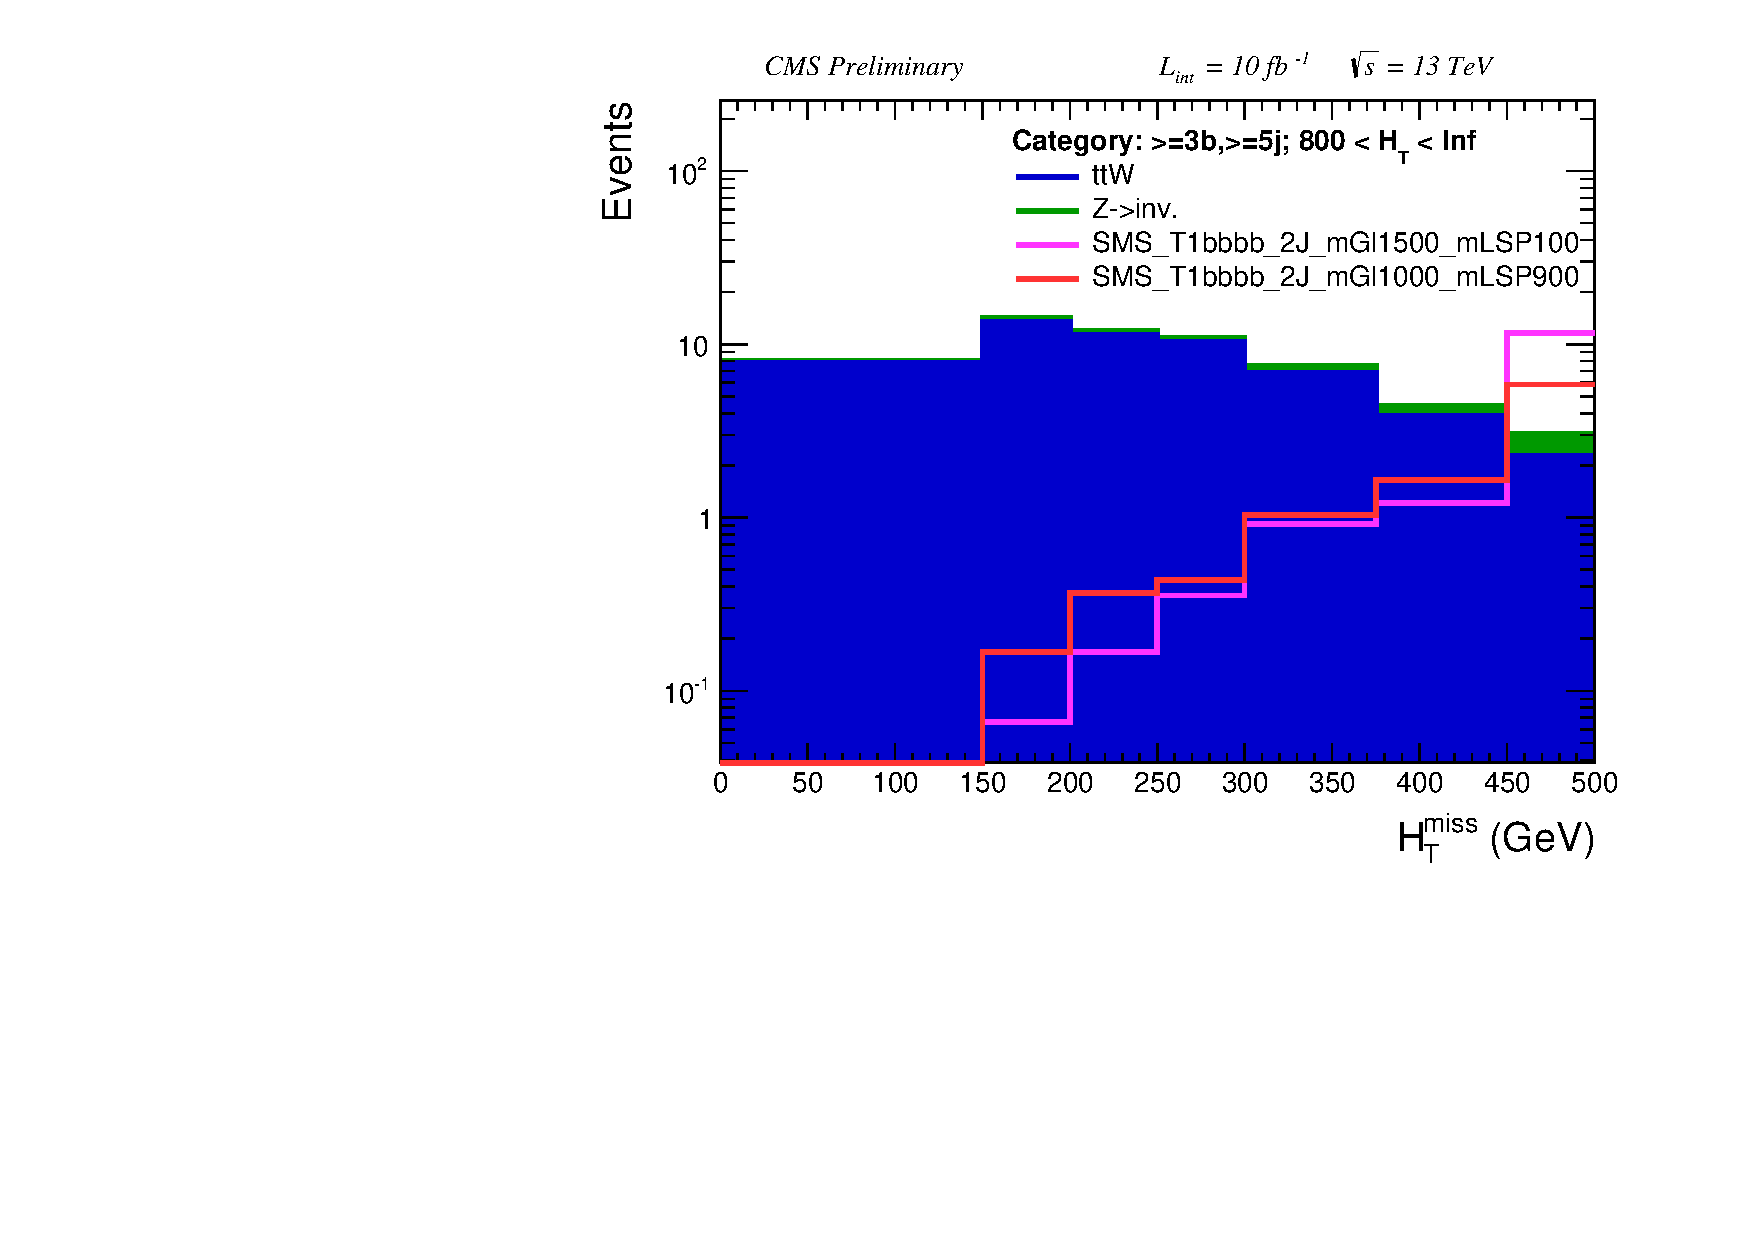
\includegraphics[width=0.5\textwidth]{figures/susyResults/MHT_ge3b_ge5j_800_Inf.pdf}}
    \caption{\mht templates for the $\njet\geq 5$, $\nb\geq 3$ category.}
    \label{fig:mht_ge3b_ge5j}
  \end{center}
\end{figure}


Table~\ref{tab:results_ul} and \ref{tab:results_signif} show, respectively, 
the expected 95\% upper limit on the signal strength $\mu=\sigma/\sigma_{\mathrm{theory}}$ 
and the expected discovery significance, for all the simplified models. 
The projections are done for an integrated luminosity of 3 \ifb and 10 \ifb. 
The effect of including a ``toy'' template uncertainty (Section \ref{sec:syst-on-shape}) is compared to the result without any template systematic.  

Both the significance and the limit are computed using the asymptotic formulae and the pre-fit Asimov datasets \cite{AsymptoticFormulae}. 
The upper limits are computed using the $\text{CL}_{s}$ criterion \cite{CLsTechnique}. \\
All the statistical results are produced using the \textit{combine} tool, 
provided within the HiggsAnalysis-CombinedLimit package \cite{Combine}. \\
For each model, the categories used in the combination are listed in table \ref{tab:simplified-models}. 

\begin{table}
  \centering
  \caption{95\% C.L. upper limit on $\mu$ for the different benchmark models and the different luminosity scenarios. 
  The main result is obtained by applying 
  the ``toy'' template systematic described in Section~\ref{sec:syst-on-shape}, 
while in parentheses the result without any template systematic is reported. 
For T2qq, two degenerate light squark generations are assumed.}
  \label{tab:results_ul}
  \footnotesize
  \begin{tabular}{lcc}
    \hline
    \hline
    Signal model & $\mathcal{L} = 3 \ifb$ & $\mathcal{L} = 10 \ifb$ \\
    \hline
    \hline
    T1bbbb 1500,100  & 0.68 (0.66) & 0.33 (0.31) \\ 
    T1bbbb 1000,900  & 0.67 (0.62) & 0.35 (0.31) \\ 
    T1qqqq 1400,100  & 0.98 (0.82) & 0.54 (0.41) \\ 
    T1qqqq 1000,800  & 0.75 (0.65) & 0.42 (0.35) \\ 
    T1tttt 1500,100  & 1.9 (1.84) & 0.92 (0.86) \\  
    T1tttt 1200,800  & 3.89 (3.78) & 2.06 (1.93) \\ \hline
    T2tt 850,100     & 2.07 (1.91) & 1.13 (0.98) \\ 
    T2tt 650,325     & 2.3 (2.16) & 1.32 (1.18) \\  
    T2tt 500,325     & 3.48 (3.39) & 1.88 (1.79) \\ 
    T2tt 425,325     & 2.16 (2.02) & 1.19 (1.1) \\  
    T2qq 1200,100    & 1.75 (1.43) & 0.91 (0.7) \\  
    T2qq 600,550     & 0.57 (0.47) & 0.32 (0.24) \\ 
    T2bb 900,100     & 4.89 (3.95) & 2.84 (2.13) \\ 
    T2bb 600,580     & 1.84 (1.71) & 0.92 (0.82) \\ 
    \hline
    \hline
  \end{tabular} 
\end{table}


\begin{table}
  \centering
  \caption{Expected significance for the different benchmark models and the different luminosity scenarios. 
    The main result is obtained by applying 
  the ``toy'' template systematic described in Section \ref{sec:syst-on-shape},
while in parentheses the result without any template systematic is reported. 
For T2qq, two degenerate light squark generations are assumed.}

  \label{tab:results_signif}
  \footnotesize
  \footnotesize
  \begin{tabular}{lcc}
    \hline
    \hline
    Signal model & $\mathcal{L} = 3 \ifb$ & $\mathcal{L} = 10 \ifb$ \\
    \hline
    \hline
    T1bbbb 1500,100  & 3.0 (3.3) & 5.2 (5.9) \\  
    T1bbbb 1000,900  & 3.0 (3.4) & 5.1 (6.2) \\  
    T1qqqq 1400,100  & 1.9 (2.6) & 3.2 (4.8) \\  
    T1qqqq 1000,800  & 2.6 (3.1) & 4.6 (5.6) \\  
    T1tttt 1500,100  & 1.3 (1.4) & 2.2 (2.5) \\  
    T1tttt 1200,800  & 0.6 (0.6) & 1.0 (1.1) \\  \hline
    T2tt 850,100     & 1.0 (1.2) & 1.8 (2.1) \\  
    T2tt 650,325     & 0.9 (1.0) & 1.5 (1.7) \\  
    T2tt 500,325     & 0.6 (0.6) & 1.1 (1.2) \\  
    T2tt 425,325     & 0.9 (1.0) & 1.7 (1.9) \\  
    T2qq 1200,100    & 1.1 (1.5) & 2.1 (2.9) \\  
    T2qq 600,550     & 3.3 (4.3) & 6.0 (8.0) \\  
    T2bb 900,100     & 0.4 (0.5) & 0.7 (1.0) \\  
    T2bb 600,580     & 1.2 (1.3) & 2.2 (2.5) \\  
    \hline
    \hline
  \end{tabular} 
\end{table}


%%____________________________________________________________________________||
